% Options for packages loaded elsewhere
\PassOptionsToPackage{unicode}{hyperref}
\PassOptionsToPackage{hyphens}{url}
\documentclass[
]{article}
\usepackage{xcolor}
\usepackage{amsmath,amssymb}
\setcounter{secnumdepth}{-\maxdimen} % remove section numbering
\usepackage{iftex}
\ifPDFTeX
  \usepackage[T1]{fontenc}
  \usepackage[utf8]{inputenc}
  \usepackage{textcomp} % provide euro and other symbols
\else % if luatex or xetex
  \usepackage{unicode-math} % this also loads fontspec
  \defaultfontfeatures{Scale=MatchLowercase}
  \defaultfontfeatures[\rmfamily]{Ligatures=TeX,Scale=1}
\fi
\usepackage{lmodern}
\ifPDFTeX\else
  % xetex/luatex font selection
\fi
% Use upquote if available, for straight quotes in verbatim environments
\IfFileExists{upquote.sty}{\usepackage{upquote}}{}
\IfFileExists{microtype.sty}{% use microtype if available
  \usepackage[]{microtype}
  \UseMicrotypeSet[protrusion]{basicmath} % disable protrusion for tt fonts
}{}
\makeatletter
\@ifundefined{KOMAClassName}{% if non-KOMA class
  \IfFileExists{parskip.sty}{%
    \usepackage{parskip}
  }{% else
    \setlength{\parindent}{0pt}
    \setlength{\parskip}{6pt plus 2pt minus 1pt}}
}{% if KOMA class
  \KOMAoptions{parskip=half}}
\makeatother
\usepackage{graphicx}
\makeatletter
\newsavebox\pandoc@box
\newcommand*\pandocbounded[1]{% scales image to fit in text height/width
  \sbox\pandoc@box{#1}%
  \Gscale@div\@tempa{\textheight}{\dimexpr\ht\pandoc@box+\dp\pandoc@box\relax}%
  \Gscale@div\@tempb{\linewidth}{\wd\pandoc@box}%
  \ifdim\@tempb\p@<\@tempa\p@\let\@tempa\@tempb\fi% select the smaller of both
  \ifdim\@tempa\p@<\p@\scalebox{\@tempa}{\usebox\pandoc@box}%
  \else\usebox{\pandoc@box}%
  \fi%
}
% Set default figure placement to htbp
\def\fps@figure{htbp}
\makeatother
\ifLuaTeX
  \usepackage{luacolor}
  \usepackage[soul]{lua-ul}
\else
  \usepackage{soul}
\fi
\setlength{\emergencystretch}{3em} % prevent overfull lines
\providecommand{\tightlist}{%
  \setlength{\itemsep}{0pt}\setlength{\parskip}{0pt}}
\ifPDFTeX
  \TeXXeTstate=1
  \newcommand{\RL}[1]{\beginR #1\endR}
  \newcommand{\LR}[1]{\beginL #1\endL}
  \newenvironment{RTL}{\beginR}{\endR}
  \newenvironment{LTR}{\beginL}{\endL}
\fi
\usepackage{bookmark}
\IfFileExists{xurl.sty}{\usepackage{xurl}}{} % add URL line breaks if available
\urlstyle{same}
\hypersetup{
  pdftitle={Image Embeddings},
  hidelinks,
  pdfcreator={LaTeX via pandoc}}

\title{Image Embeddings}
\author{}
\date{}

\begin{document}
\maketitle

\begin{verbatim}
#### Embeddings
\end{verbatim}

Representation of input data as points within a continuous vector space

\url{https://projector.tensorflow.org/}\strut \\
\pandocbounded{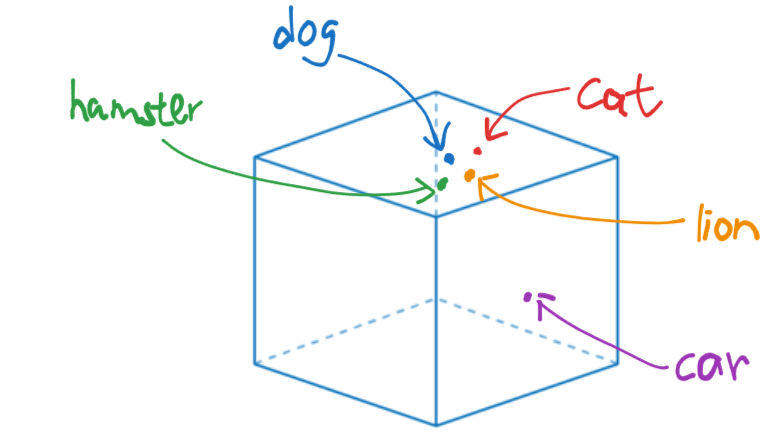
\includegraphics[keepaspectratio]{C:/Users/v4m5HSjp7tk/Documents/YEWTEEBEE/msc/notes/Project Ideas/Pasted image 20250213032451.png}}

There are many ways of encoding or representing the input data

\subsubsection{Pretrained Feature
Embeddings}\label{pretrained-feature-embeddings}

\paragraph{Transfer Learning}\label{transfer-learning}

A network pretrained on a very large dataset learn rich representations
of visual data\\
-\textgreater{} Fine-tuning on this allows the model to adapt and learn
new features regarding the task more quickly\\
-\textgreater{} Activations of a deeper layer of a pretrained model
serve as embeddings that represent features of the image in a more
informative space

\begin{center}\rule{0.5\linewidth}{0.5pt}\end{center}

transfer learning + vanilla model = baseline embedding used in FYP

\subsubsection{Latent Space Representations (Autoencoders or
VAEs)}\label{latent-space-representations-autoencoders-or-vaes}

\paragraph{Autoencoders}\label{autoencoders}

Learn compressed representation of raw data

\begin{itemize}
\tightlist
\item
  More concretely, learn good lower-dimensional representation of the
  dataset
\end{itemize}

Two parts:\\
1.Encoder

\begin{itemize}
\tightlist
\item
  Deterministically (same output for given input always) maps data to a
  representation space\\
  2.Decoder
\item
  Maps representation space back to original data space
\end{itemize}

\pandocbounded{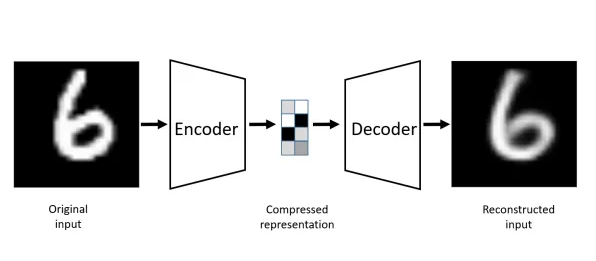
\includegraphics[keepaspectratio]{C:/Users/v4m5HSjp7tk/Documents/YEWTEEBEE/msc/notes/Project Ideas/Pasted image 20250212153409.png}}\\
\pandocbounded{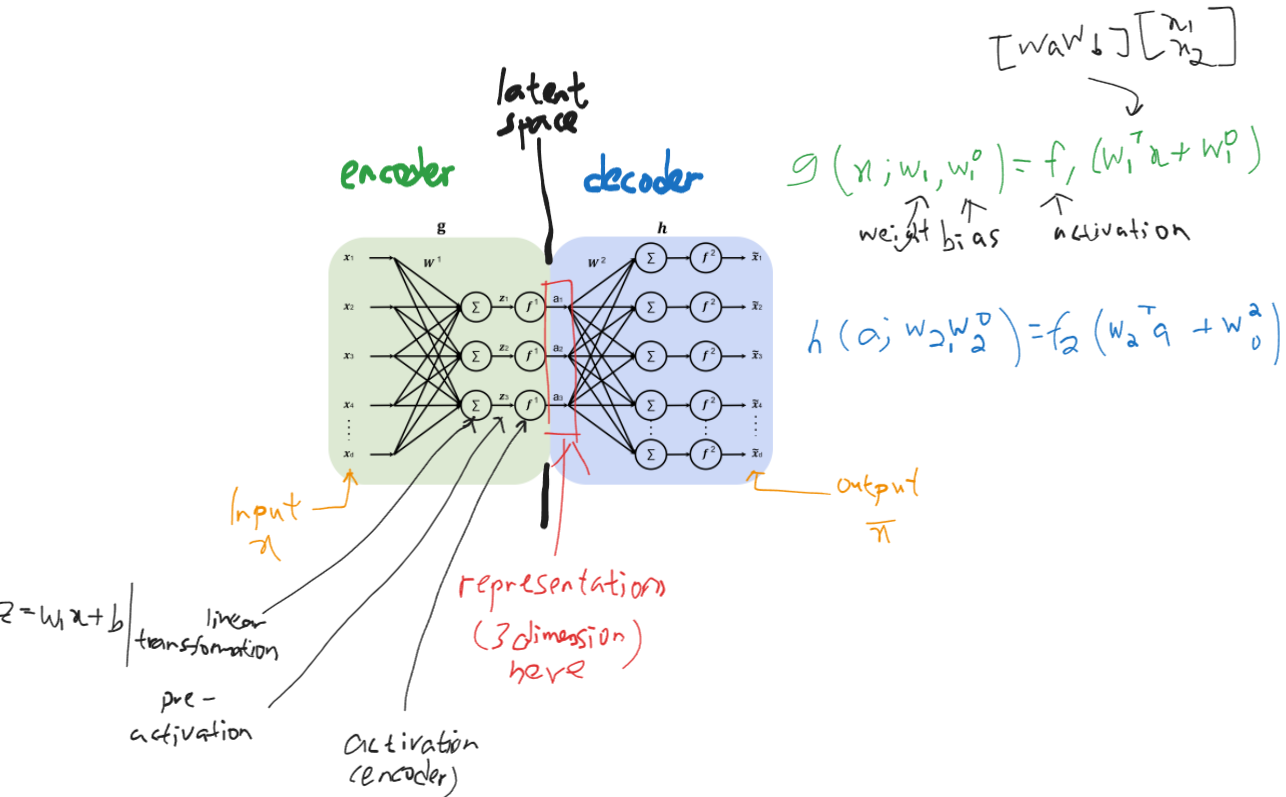
\includegraphics[keepaspectratio]{C:/Users/v4m5HSjp7tk/Documents/YEWTEEBEE/msc/notes/Project Ideas/Pasted image 20250212134824.png}}

Bottleneck

\begin{itemize}
\tightlist
\item
  Created by having dimension of representation (a) smaller than input
  (x), resulting in dimensionality reduction
\end{itemize}

During Training:-

\begin{enumerate}
\tightlist
\item
  Data gets encoded and decoded in each pass
\item
  Reconstruction loss determines how much the output differs from the
  input
\item
  Minimize loss with backpropagation
\end{enumerate}

\begin{itemize}
\tightlist
\item
  Goal is to reconstruct the output as closely as possible given an
  encoded representation of the input
\end{itemize}

\paragraph{How can it improve
classification?}\label{how-can-it-improve-classification}

Why even use autoencoders for classification?

\begin{itemize}
\tightlist
\item
  Bottleneck effect reduces input dimensionality

  \begin{itemize}
  \tightlist
  \item
    -\textgreater{} Helps when input dimensions is too large for model
  \item
    -\textgreater{} Ideally, it learns the most important features of
    the input data
  \item
    -\textgreater{} Ideally less memorization, more robust
  \end{itemize}
\end{itemize}

\paragraph{Autoencoder for
Classification}\label{autoencoder-for-classification}

\begin{enumerate}
\tightlist
\item
  Autoencoder (with bottleneck) first trained normally to learn
  compressed latent representation
\item
  Decoder is replaced with another classifier model
\item
  Compressed representations used as input to classifier model
\end{enumerate}

\paragraph{Additional Types of
Autoencoder}\label{additional-types-of-autoencoder}

\subparagraph{Sparse Autoencoder}\label{sparse-autoencoder}

Different way of bottlenecking

\begin{itemize}
\tightlist
\item
  \begin{enumerate}
  \tightlist
  \item
    Keep the number of dimensions high
  \end{enumerate}
\item
  \begin{enumerate}
  \setcounter{enumi}{1}
  \tightlist
  \item
    Introduce sparsity by constraining neurons to be inactive most of
    the time
  \end{enumerate}
\item
  -\textgreater{} Similar concept as regularization
\item
  -\textgreater{} Usually results in more interpretable features, better
  for anomaly detection
\end{itemize}

\pandocbounded{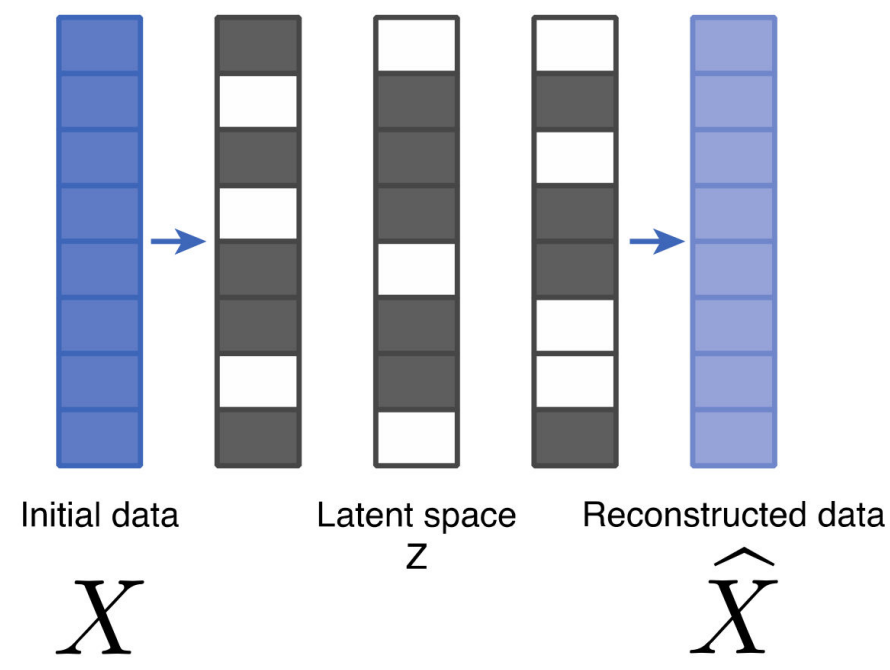
\includegraphics[keepaspectratio]{C:/Users/v4m5HSjp7tk/Documents/YEWTEEBEE/msc/notes/Project Ideas/Pasted image 20250213114231.png}}

\subparagraph{Variational Autoencoder}\label{variational-autoencoder}

Probabilistic rather than deterministic

\begin{itemize}
\tightlist
\item
  encode latent variables of training data not as a fixed discrete
  value, but as a continuous range of possibilities expressed as a
  probability distribution
\end{itemize}

Bottleneck is typically modeled as a lower dimensional latent space
\textbf{with} Gaussian distribution of mean \emph{μ} vectors~and σ{}
variance vectors\\
-\textgreater{} Sample of this distribution is fed into decoder

\pandocbounded{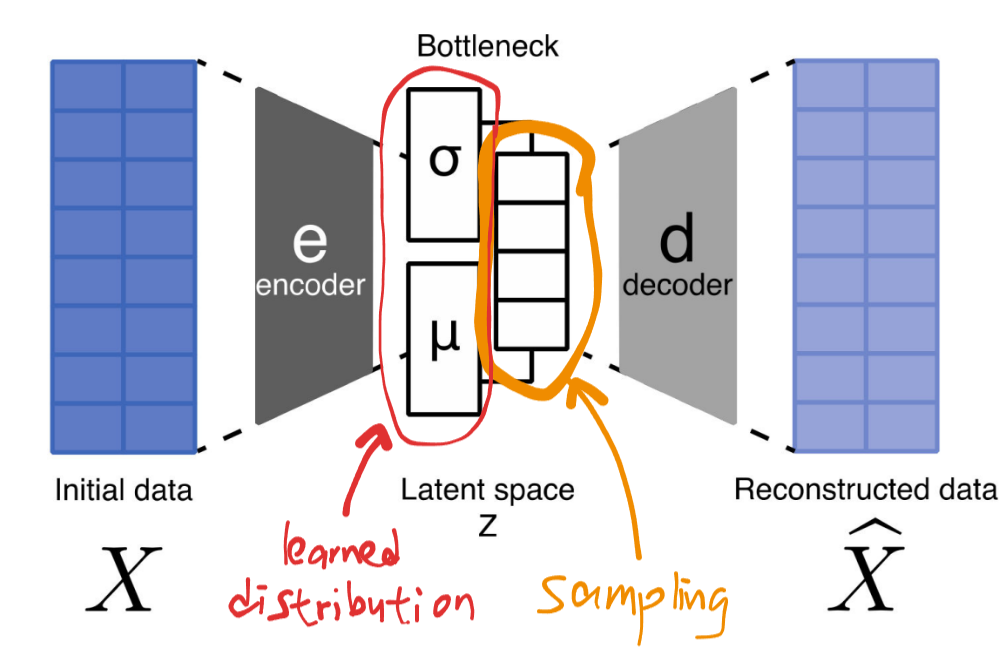
\includegraphics[keepaspectratio]{C:/Users/v4m5HSjp7tk/Documents/YEWTEEBEE/msc/notes/Project Ideas/Pasted image 20250213154252.png}}

What are we trying to learn with this distribution?

-\textgreater{} We are actually modelling the noise that is present in
the dataset

\begin{itemize}
\tightlist
\item
  Ideally, given a dataset of faces, the encoder encodes facial
  structure and features, the learned distribution represents lighting
  or saturation variations
\end{itemize}

How do we backpropagate since the sampling is probabilistic (has
randomness)?

\begin{itemize}
\tightlist
\item
  \textbf{\emph{Issue 1: Sampling is random, therefore
  non-differentiable}}

  \begin{itemize}
  \tightlist
  \item
    Lets say you wanna train a robot leg to score a goal. You missed the
    first time with 120N of force, then scored with 140N of force.
    However, you forgot to account for the stronger wind in the first
    kick, thus cannot establish a relationship between force and scoring
    accuracy. You thus need a \textbf{controlled} way of kicking the
    ball.\\
    \pandocbounded{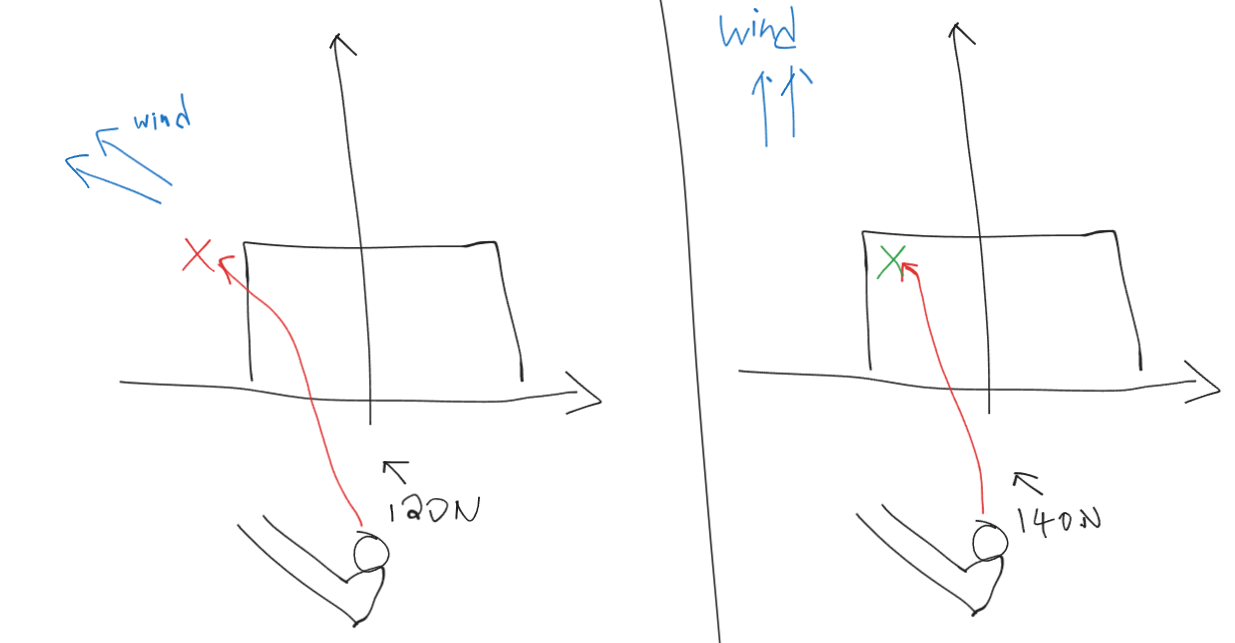
\includegraphics[keepaspectratio]{C:/Users/v4m5HSjp7tk/Documents/YEWTEEBEE/msc/notes/Project Ideas/image-1.png}}
  \item
    -\textgreater Why not take an average of many samples?

    \begin{itemize}
    \tightlist
    \item
      Expensive to run decoder multiple times
    \item
      We lose variance information

      \begin{itemize}
      \tightlist
      \item
        Results in many reconstructions
      \item
        Each sample is meant to capture different possible "versions" of
        the data
      \item
        Each reconstruction corresponds to an average sample, nuance
        lost
      \end{itemize}
    \end{itemize}
  \item
    \textbf{\emph{Issue 2: Changing the parameters affect the sample}}

    \begin{itemize}
    \tightlist
    \item
      You are in a controlled environment now and found the ideal force
      to kick the ball. This time, there is now a goalkeeper tasked with
      blocking the shot. In its first shot, the goalkeeper made a save,
      and now the robot is making a slight adjustment by shooting more
      to the right. However, the goalkeeper anticipated where the robot
      would shoot based on the first shot and blocked the shot again.
      Since the goalkeeper\textquotesingle s judgement \textbf{is
      dependent on} where the robot was aiming, we don\textquotesingle t
      know how much adjusting the shot slightly to the right improved
      the scoring chances. You thus need a way to retain information
      about the previous shot when determining scoring chances.\\
      \pandocbounded{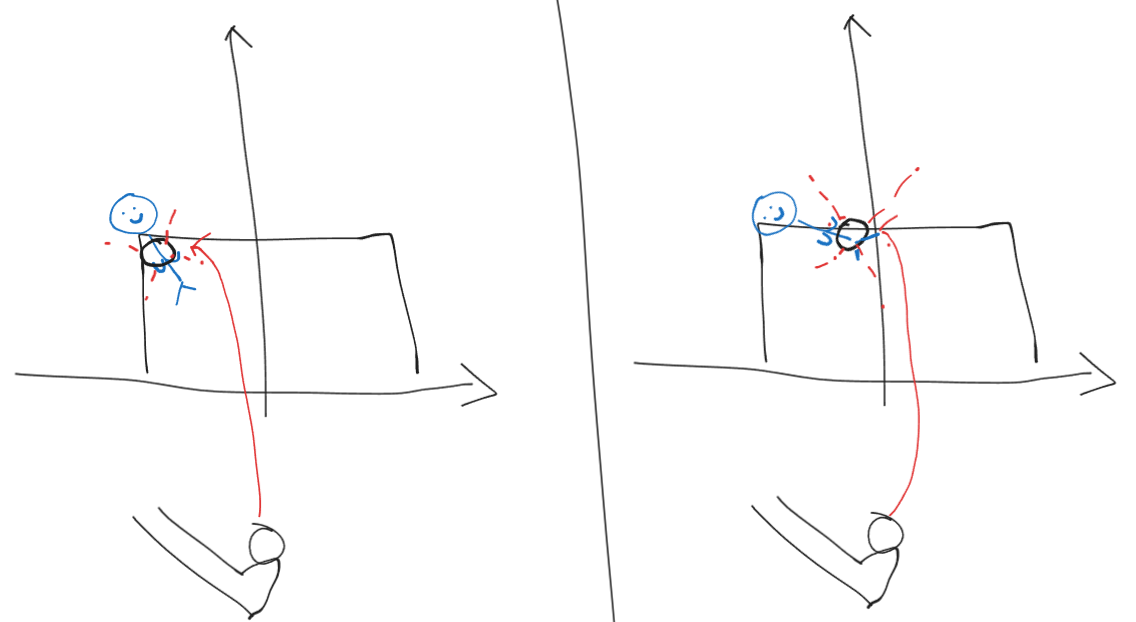
\includegraphics[keepaspectratio]{C:/Users/v4m5HSjp7tk/Documents/YEWTEEBEE/msc/notes/Project Ideas/image-3.png}}
    \end{itemize}
  \end{itemize}
\end{itemize}

mathematical justification:
\url{https://gregorygundersen.com/blog/2018/04/29/reparameterization/}

\textbf{Solution: Reparameterization Trick}\\
Express the random sampling as a separate function\\
-\textgreater mean and variance from learned distribution can be updated
in backpropagation, ϵ stays the same in a single forward and backward
pass\\
1. Allows us to calculate how learned distribution changes while
retaining information about the "sample" in the backward pass\\
2. Breaks the correlation of the of sampling on mean and variance

\pandocbounded{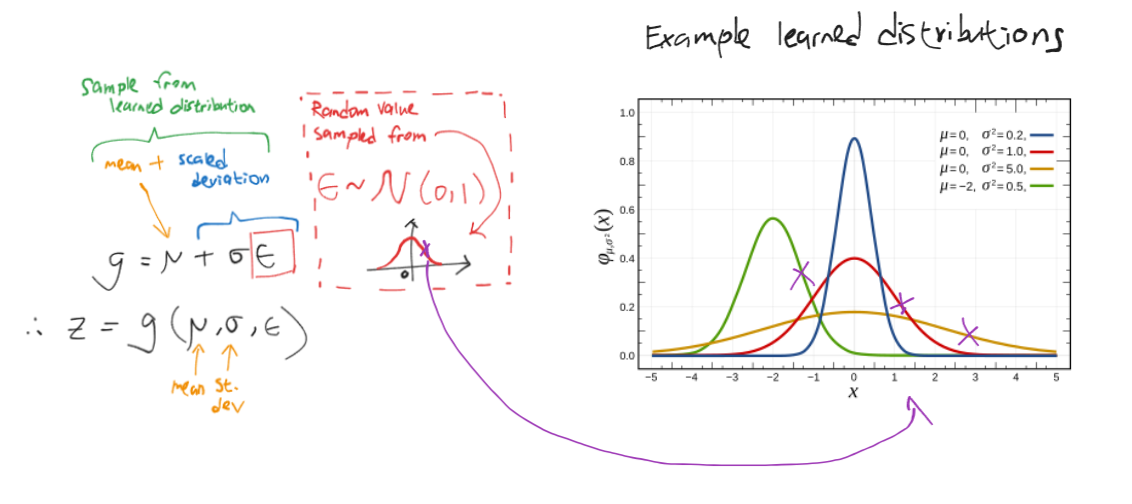
\includegraphics[keepaspectratio]{C:/Users/v4m5HSjp7tk/Documents/YEWTEEBEE/msc/notes/Project Ideas/image-7.png}}\\
\pandocbounded{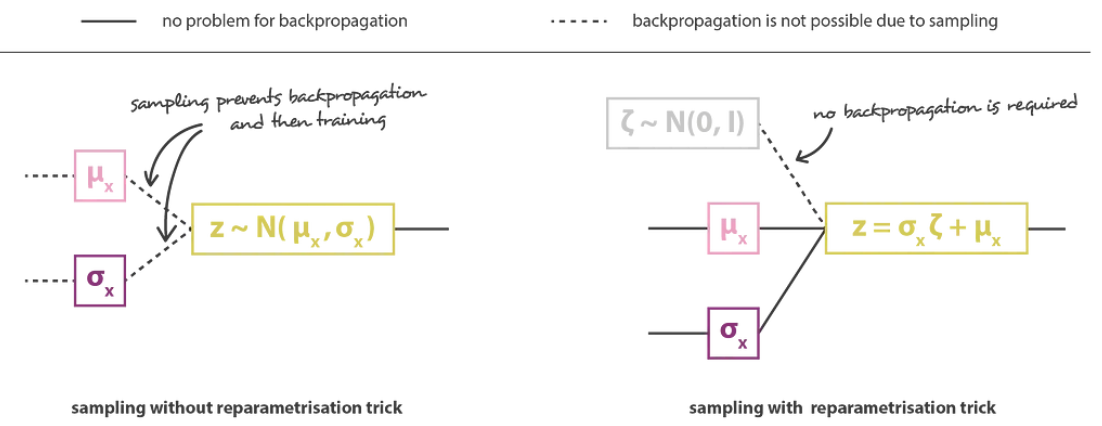
\includegraphics[keepaspectratio]{C:/Users/v4m5HSjp7tk/Documents/YEWTEEBEE/msc/notes/Project Ideas/image-5.png}}

Loss Function

Loss has two components: 1. Reconstruction Loss 2. KL Divergence
(ensures normally distributed)\\
\pandocbounded{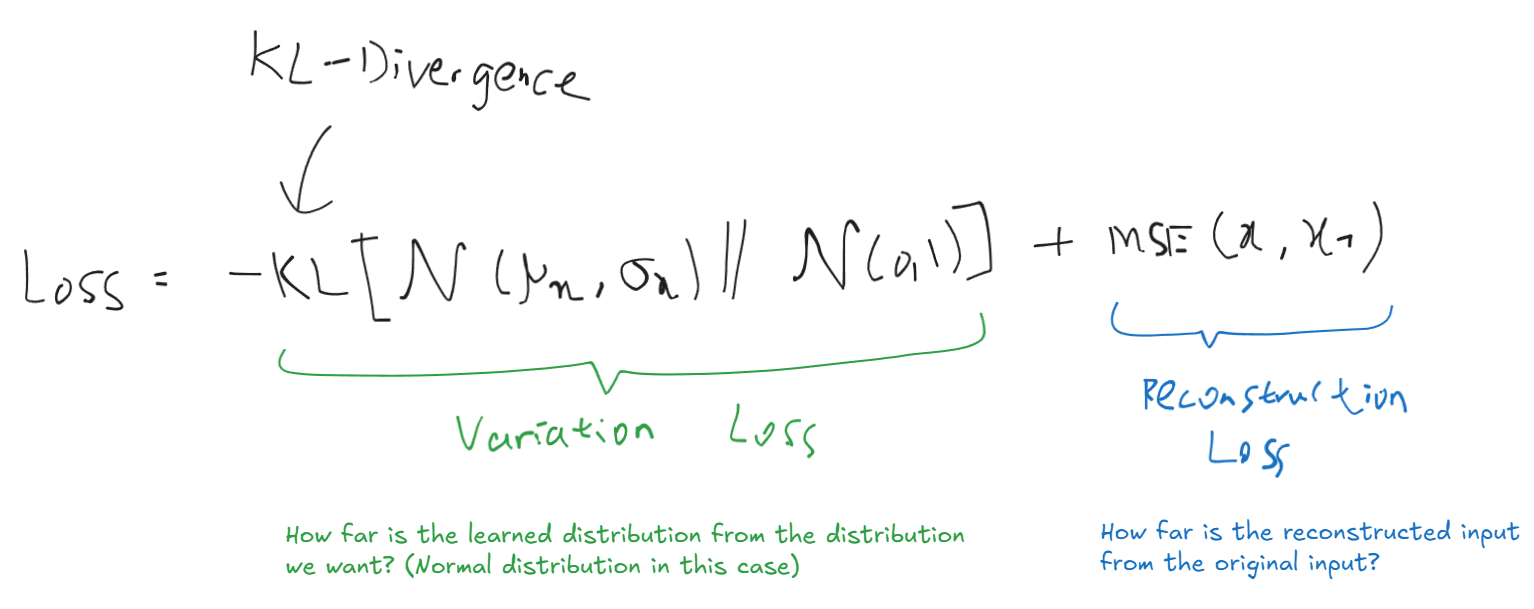
\includegraphics[keepaspectratio]{C:/Users/v4m5HSjp7tk/Documents/YEWTEEBEE/msc/notes/Project Ideas/image-9.png}}

Weighing of each loss differently has trade-offs\\
\pandocbounded{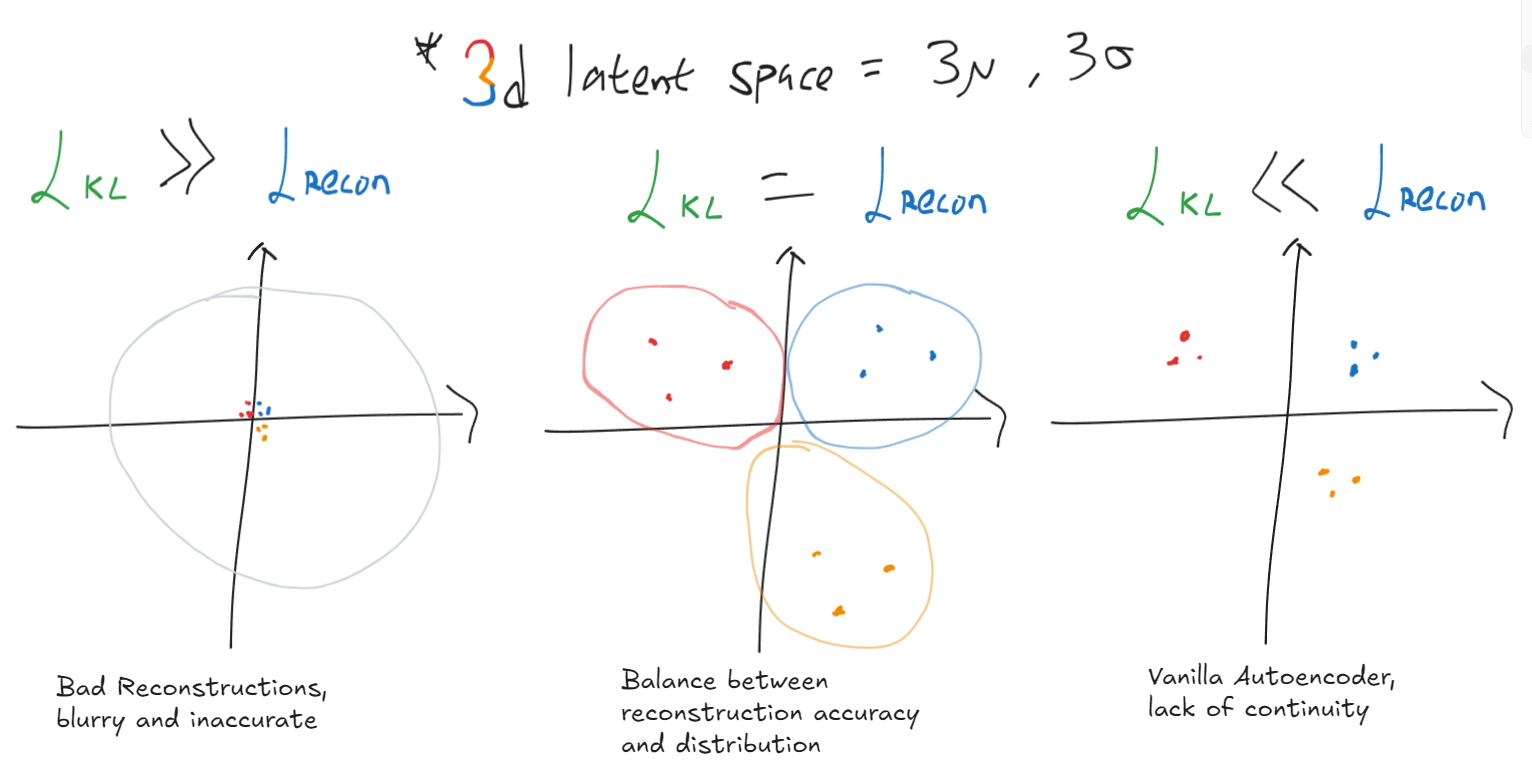
\includegraphics[keepaspectratio]{C:/Users/v4m5HSjp7tk/Documents/YEWTEEBEE/msc/notes/Project Ideas/image-11.png}}

During training:-

\begin{enumerate}
\tightlist
\item
  Input x gets encoded
\item
  d (number of dimensions) means and variances (learned distributions)
  that corresponds to this x is determined
\item
  Random samples z to z{} taken from d learned distributions
\item
  Decoder reconstructs based on z values
\item
  Loss is calculated based on z values, means and variances also to be
  adjusted
\item
  Minimize loss using backpropagation
\end{enumerate}

\pandocbounded{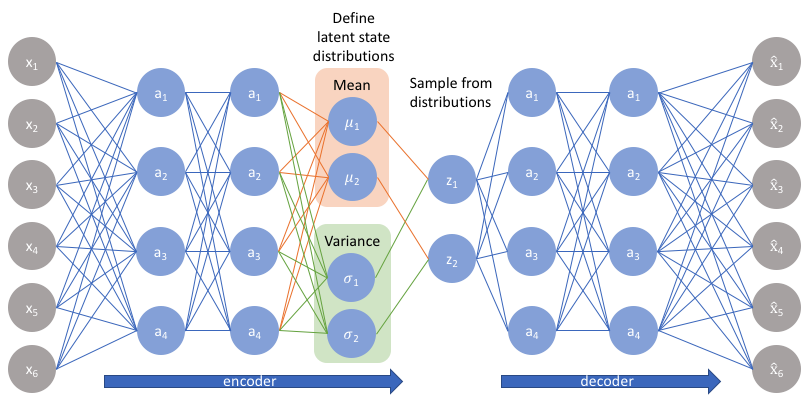
\includegraphics[keepaspectratio]{C:/Users/v4m5HSjp7tk/Documents/YEWTEEBEE/msc/notes/Project Ideas/image-14.png}}

Why VAE over vanilla AE?

\begin{enumerate}
\item
  Continuity\\
  Can sample over any point, has meaningful interpolations and smooth
  transformations\\
  -\textgreater e.g., morphing one face into another\\
  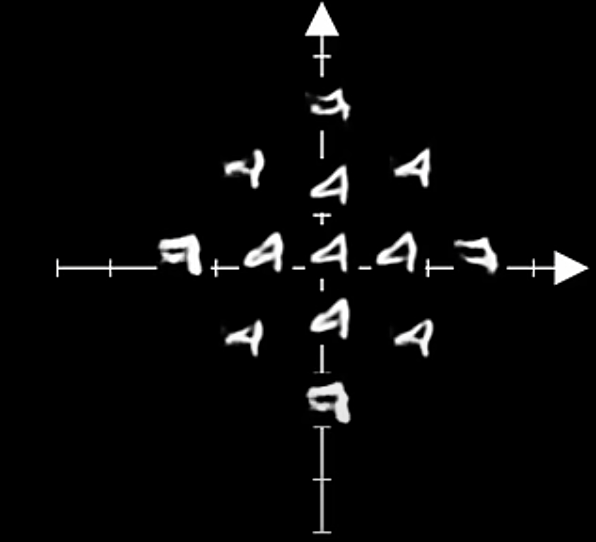
\includegraphics[width=2.97917in,height=2.70833in]{C:/Users/v4m5HSjp7tk/Documents/YEWTEEBEE/msc/notes/Project Ideas/image-12.png}
\item
  Noise is controlled\\
  You force the model to recognize noise, ideally making the model
  generalize better
\item
  Structured Learning\\
  Disentangled Representations: You force the learning of structured
  latent spaces where each dimension captures a distinct factor.
\end{enumerate}

\subparagraph{Masked Autoencoder}\label{masked-autoencoder}

Input data is partially masked or corrupted before being fed into the
autoencoder

\pandocbounded{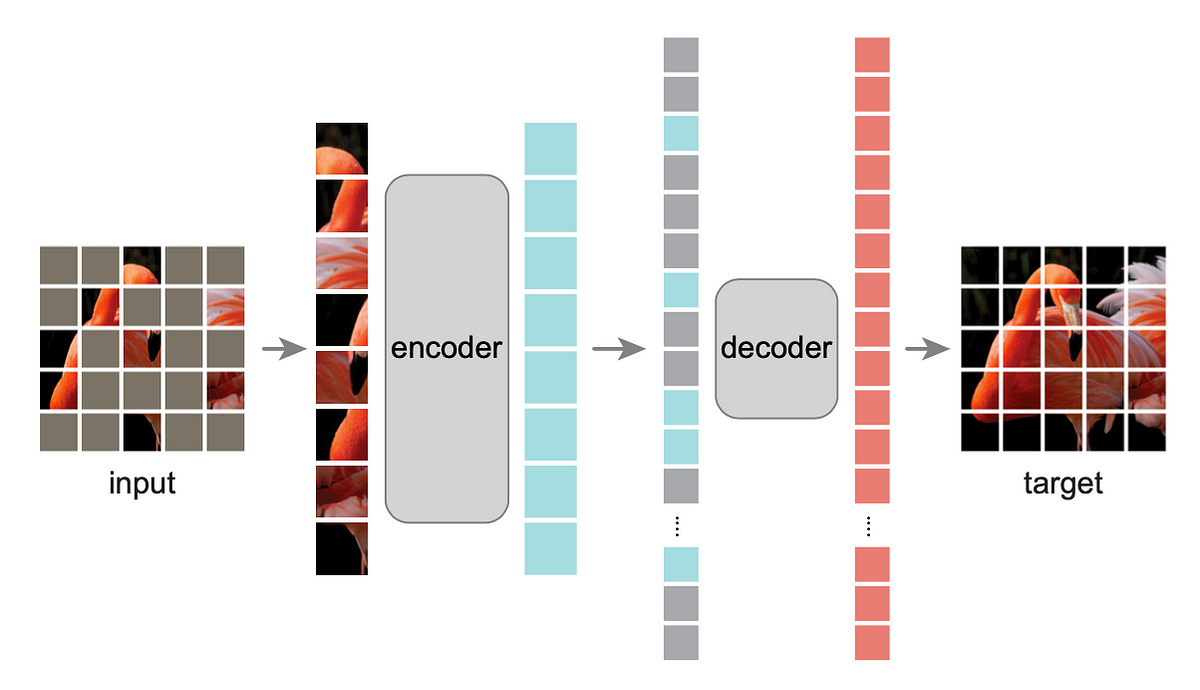
\includegraphics[keepaspectratio]{C:/Users/v4m5HSjp7tk/Documents/YEWTEEBEE/msc/notes/Project Ideas/Pasted image 20250213110604.png}}

\textbf{Some stuff to think about:}

\begin{enumerate}
\tightlist
\item
  Words are discrete, image space is continuous (rgb values)
\item
  Information density in language vs images is very different

  \begin{itemize}
  \tightlist
  \item
    Obscuring a random word in a sentence vs obscuring random pixels in
    an image
  \end{itemize}
\item
  1 pixel has little to no information, a collection of pixels can be
  contextually significant (0,0,255 vs blueberry)\\
  \pandocbounded{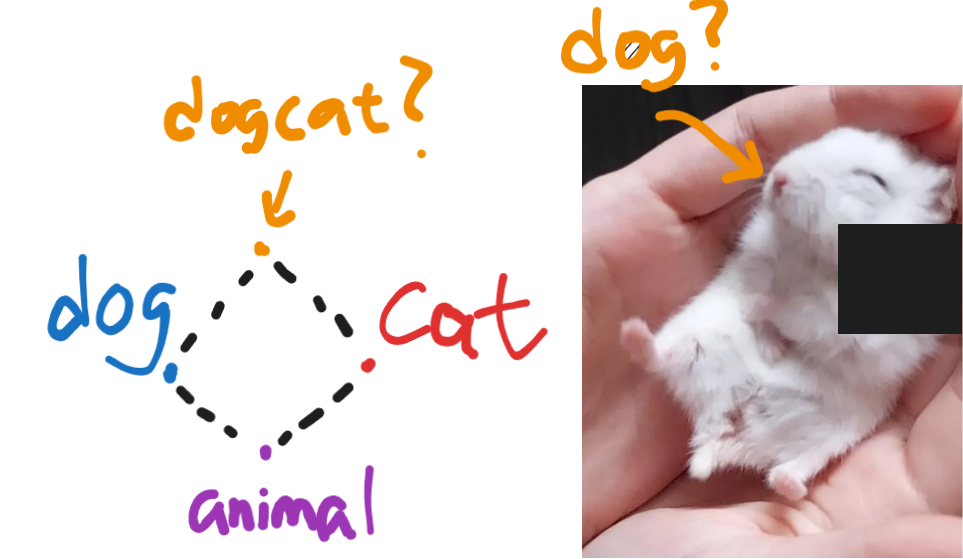
\includegraphics[keepaspectratio]{C:/Users/v4m5HSjp7tk/Documents/YEWTEEBEE/msc/notes/Project Ideas/Pasted image 20250213035754.png}}
\end{enumerate}

Masked Autoencoders are Scalable Vision Learners\\
\url{https://arxiv.org/pdf/2111.06377}

Apparently we can remove 75\% of the input image for a ViT-based
encoder-decoder network and still get a relatively decent
reconstruction\\
-\textgreater{} Transformer decoder means that positional embeddings are
used, still there is additional position context for each patch (square
block below)

Pretraining on masked autoencoder improved larger ViT models, suggesting
that it helps solve overfitting and scale up model sizes

\pandocbounded{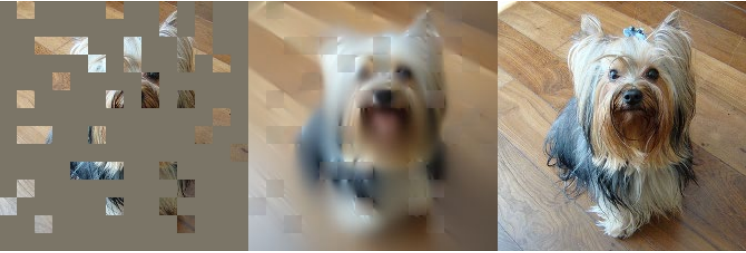
\includegraphics[keepaspectratio]{C:/Users/v4m5HSjp7tk/Documents/YEWTEEBEE/msc/notes/Project Ideas/Pasted image 20250213040344.png}}

\subsubsection{Attention-Based
Embeddings}\label{attention-based-embeddings}

Positional information is added to the embedding

Transformer neural networks use multiple encoder and decoder blocks,
together with a\\
self-attention mechanism. Vanilla Vision Transformers (for image
classification) have no decoder, i.e., they are decoder-only, we are
just getting the embeddings from the encoder and feeding into the
classifier network.

\paragraph{Patch Embedding}\label{patch-embedding}

Image is first split into patches.\\
Note: in vanilla ViT, patches are non-overlapping\\
\pandocbounded{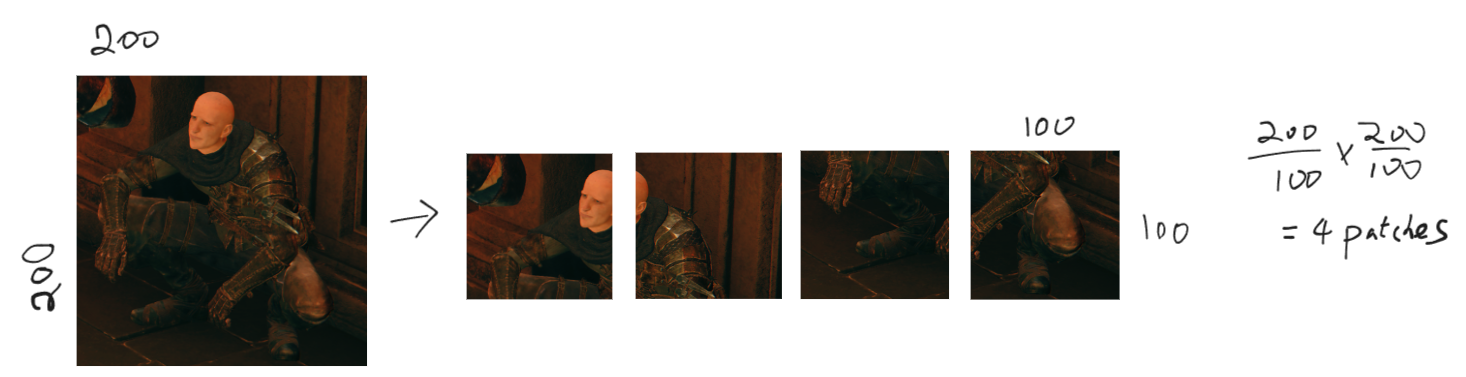
\includegraphics[keepaspectratio]{C:/Users/v4m5HSjp7tk/Documents/YEWTEEBEE/msc/notes/Project Ideas/image-18.png}}

Patches flattened to 1D vector. 3 Channels (r,g,b) combined.\\
\pandocbounded{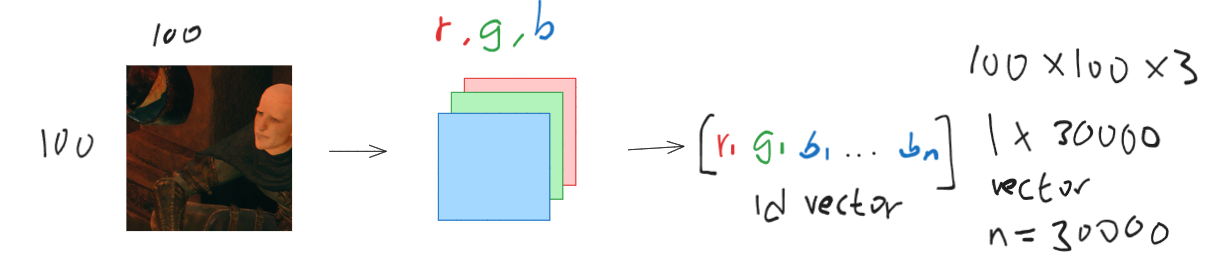
\includegraphics[keepaspectratio]{C:/Users/v4m5HSjp7tk/Documents/YEWTEEBEE/msc/notes/Project Ideas/image-30.png}}

Linear projection is performed (each new feature is simple a weighted
sum of the original features).\\
Note: in vanilla ViT, D is the same dimension as the 1d vector (also
allows for easier implementation of skip connections)\\
\pandocbounded{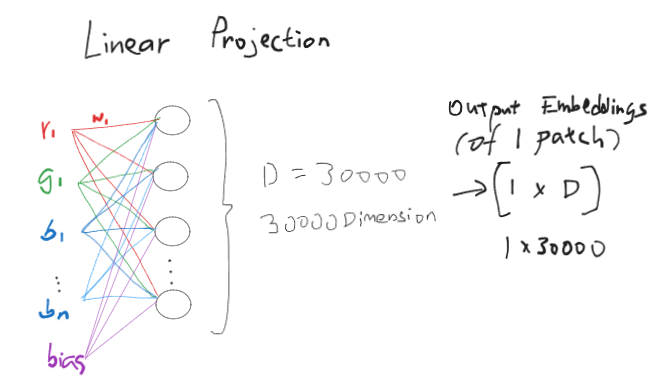
\includegraphics[keepaspectratio]{C:/Users/v4m5HSjp7tk/Documents/YEWTEEBEE/msc/notes/Project Ideas/image-45.png}}

\paragraph{Positional Embedding}\label{positional-embedding}

We want to retain information on where the position of each patch is in
the image.\\
But why a separate encoding? Why can\textquotesingle t linear projection
alone encode spatial order?\\
-\textgreater Attention has no notion of space innately. The linear
projection step only maps pixel values into a latent space. The same
linear projection is applied to any individual patch. Even if you
shuffle the patches, each patch would be treated the same way. Need a
way to add positional information to our patch embeddings.

\textbf{Learned 1D Positional Encoding}\\
Positional information is encoded as a learnable "lookup table". Not a
neural network per se as it has no input, but instead treated as a
learnable parameter backpropagated via the overall task loss
(classification loss).

\textbf{What does 1D mean? Why not 2D?}\\
1D encoding can be seen as "Patch 1 is Position 1, Patch 2 is Position
2", 2D encoding can be seen as "Patch 1 is at (0,0), Patch 2 is at
(1,0)". The original ViT paper mentioned that there was no difference in
performance between 1D and 2D.

\textbf{Why learnable embeddings?}\\
Traditionally positional information in Transformers are encoded (with
sinusoidal encoding) from the input rather than learned from scratch.
While learnable embedding and fixed encoding aims to learn patch
position, ideally making it learnable lets~the model learn what it wants
to learn and not to pollute it too much with inductive bias. Learnable
positional embeddings are more flexible and adapt based on the data and
task.

\pandocbounded{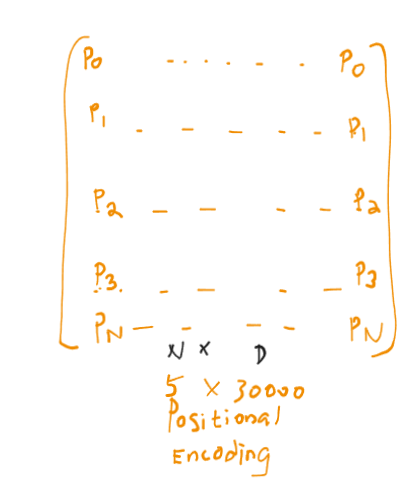
\includegraphics[keepaspectratio]{C:/Users/v4m5HSjp7tk/Documents/YEWTEEBEE/msc/notes/Project Ideas/image-46.png}}

\textbf{What does it look like?}\\
During training, these embeddings converge into vector spaces where they
show~\emph{high similarity}~to their neighboring position embeddings.
Thus, ViT\textquotesingle s positional embedding learns absolute
positioning of each patch in the image.\\
\pandocbounded{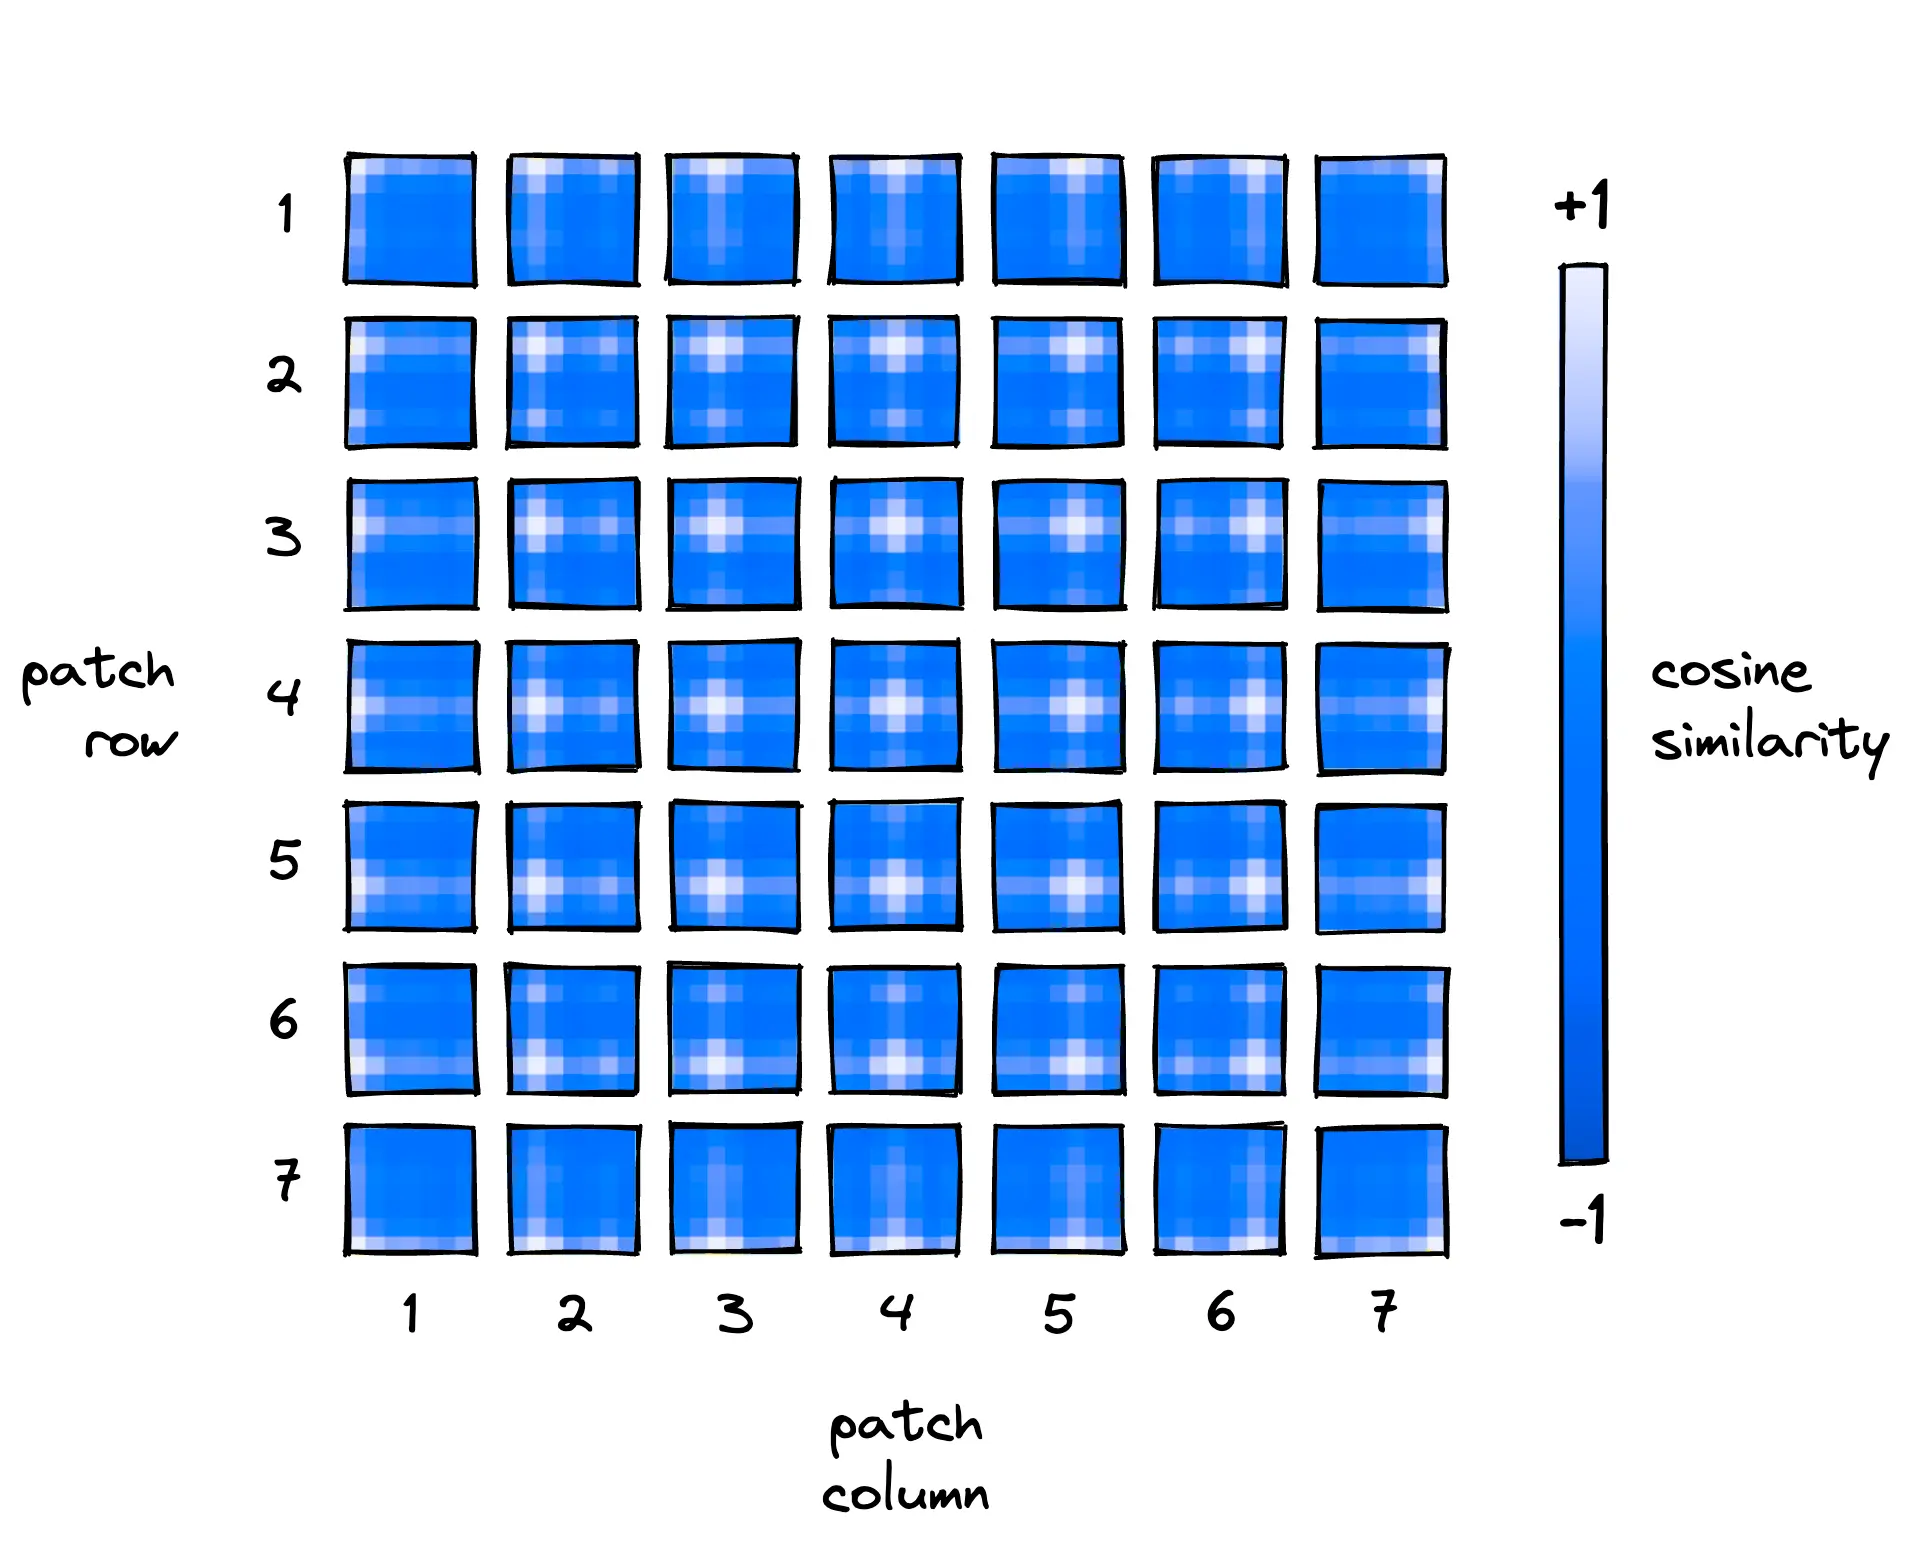
\includegraphics[keepaspectratio]{C:/Users/v4m5HSjp7tk/Documents/YEWTEEBEE/msc/notes/Project Ideas/image-37.png}}

\subparagraph{CLS Token}\label{cls-token}

\texttt{CLS} token is a "dummy" (no input) patch added to the sequence
of patch embeddings. Used for aggregating information from all the
patches. The \texttt{CLS} token is fed into the classifier network
rather than the embedding of the whole image to classify the image.

Therefore number of tokens N = Number of patches + 1\\
\pandocbounded{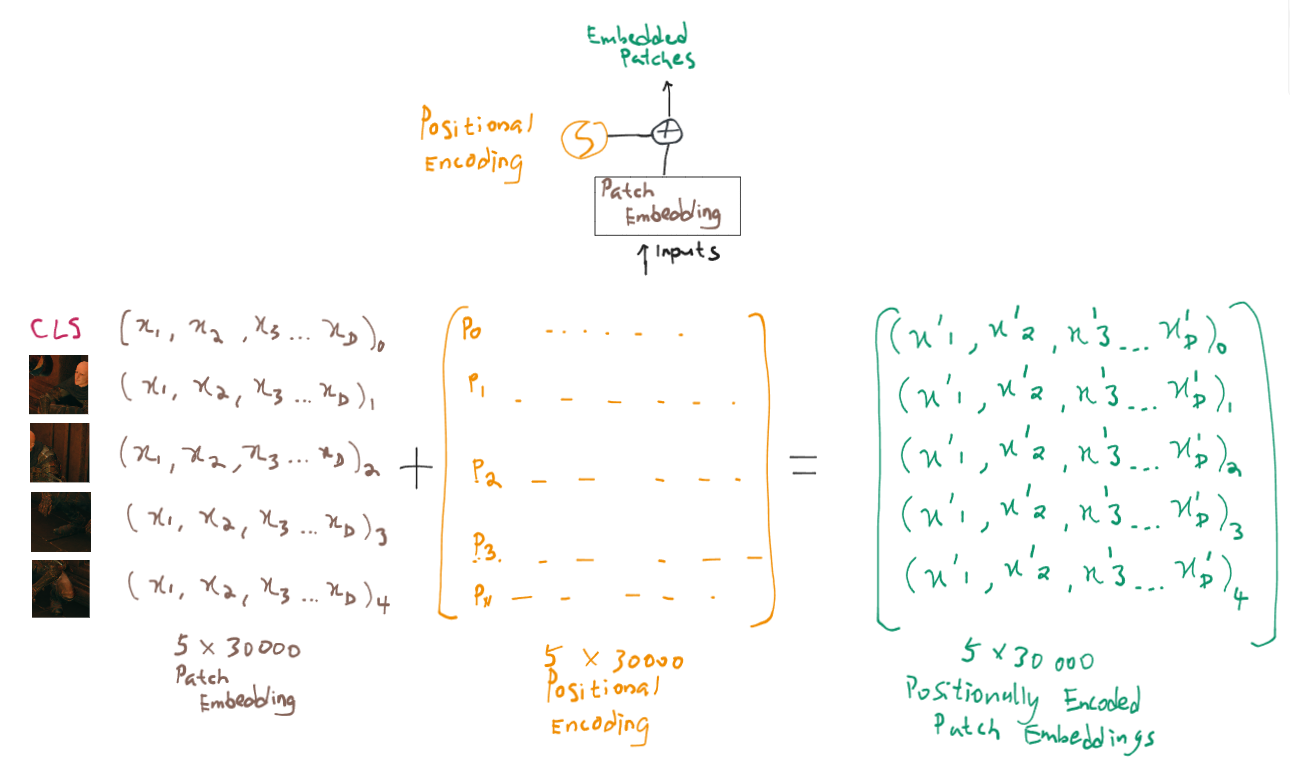
\includegraphics[keepaspectratio]{C:/Users/v4m5HSjp7tk/Documents/YEWTEEBEE/msc/notes/Project Ideas/image-48.png}}\\
Together, they make up the embedded patches

\paragraph{Transformer Encoder Block}\label{transformer-encoder-block}

\pandocbounded{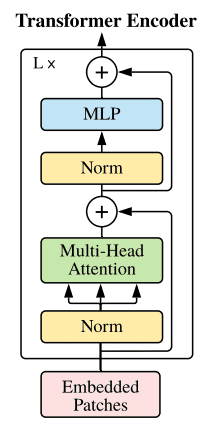
\includegraphics[keepaspectratio]{C:/Users/v4m5HSjp7tk/Documents/YEWTEEBEE/msc/notes/Project Ideas/image-81.png}}

\subparagraph{Self-Attention}\label{self-attention}

Vision transformers use self-attention to weigh the importance of each
image patch relative to one another. There any many ways to implement
attention, "self" refers to the model comparing attention scores of
elements in the input \textbf{against each other}.

Rather than just relying on local relationships (I detect a pedestrian),
this allows each element to incorporate global context (I detect a
pedestrian on a zebra crossing).

We can express how much attention each patch should give to other by
creating a lookup table of Tokens x Tokens containing attention scores.

Attention scores determine how much each patch should pay attention to
every other patch. But what do we determine if a patch is important to
another patch? What do we even compare? What do we look for? How much of
it needs to be there?

Query, Key and Value

We can express these comparative requirements into 3 parts:

\begin{enumerate}
\tightlist
\item
  The important list of features that a patch looks for in others is
  called a \textbf{Query}
\item
  The descriptive list of all the features that a certain patch contains
  is called a \textbf{Key}
\item
  The things that a patch would want to tell a certain other patch is
  called a \textbf{Value}
\end{enumerate}

\textbf{How do we obtain Query, key and value?}\\
We multiply the embedded patches with a learnable query weights vector
to obtain the query matrix (linear layer).\\
Same process occurs for the key and value vectors.\\
Typically, the dimension D of the embedded patches \textgreater{} d{}
\textgreater{} d{} = d{}\\
But in ViT, dimension D of the embedded patches \textgreater{} d{} = d{}
= d{}

\pandocbounded{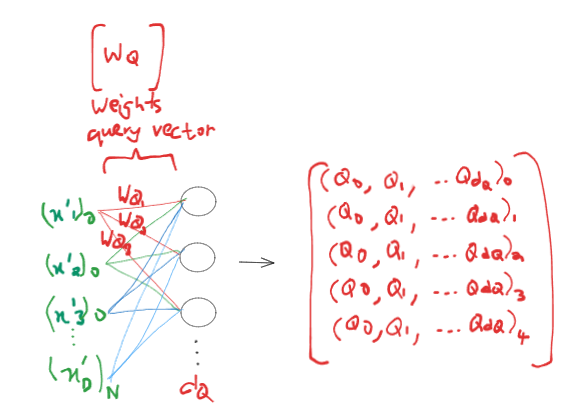
\includegraphics[keepaspectratio]{C:/Users/v4m5HSjp7tk/Documents/YEWTEEBEE/msc/notes/Project Ideas/image-60.png}}\\
\pandocbounded{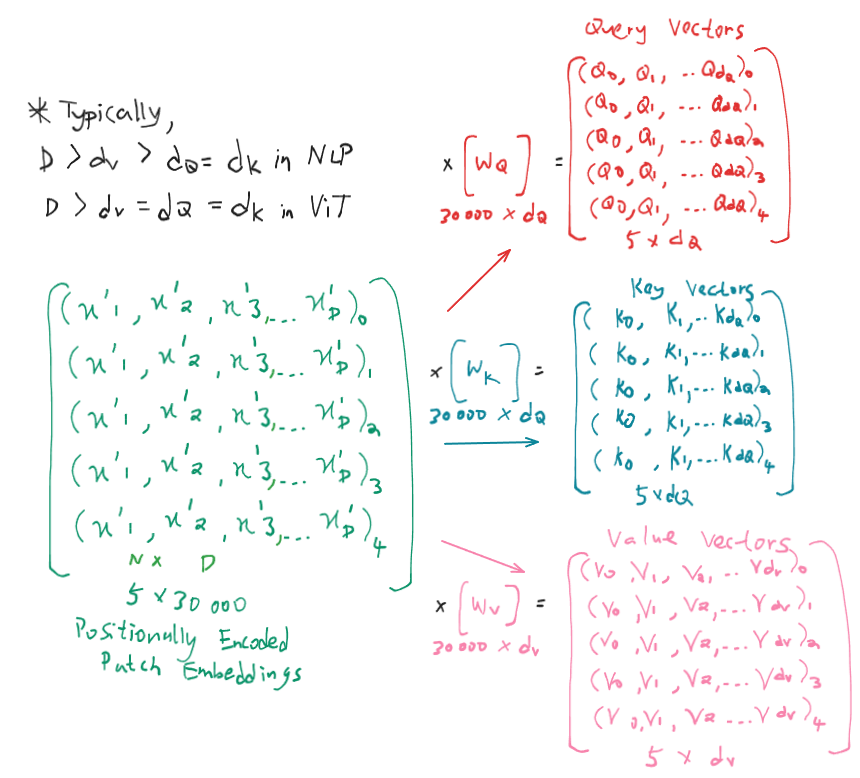
\includegraphics[keepaspectratio]{C:/Users/v4m5HSjp7tk/Documents/YEWTEEBEE/msc/notes/Project Ideas/image-77.png}}

\textbf{We can sort of gain the intuition for Q, K and V by giving it an
analogy: -}\\
Let\textquotesingle s say you are looking for a romantic partner in a
speed dating event. You interact with all the participants, looking for
suitable matches. Since you have limited time, you can only focus on a
small number of participants. In this case:

\textbf{Query:} You are actively searching for someone who matches your
ideal type. You like funny, tall and muscular men.\\
\textbf{Key:} One of the participants describe themselves as kind,
ambitious and calm. This man is well-built and 190cm tall. You compare
this person's traits to your preferences.\\
\textbf{Attention score:} Based on comparing this
participant\textquotesingle s traits with your ideal type, you choose to
focus on interacting with him more than the other participants.\\
\textbf{Value:} You both discuss what each other brings to the
relationship. Since you are interested in this person, you listen and
pay more attention to what he has to say (his job, his background, his
temperament, your chemistry together, etc.). At the end of the day,
these conversations contain the content that helps you decide whether or
not to pursue this relationship.

\pandocbounded{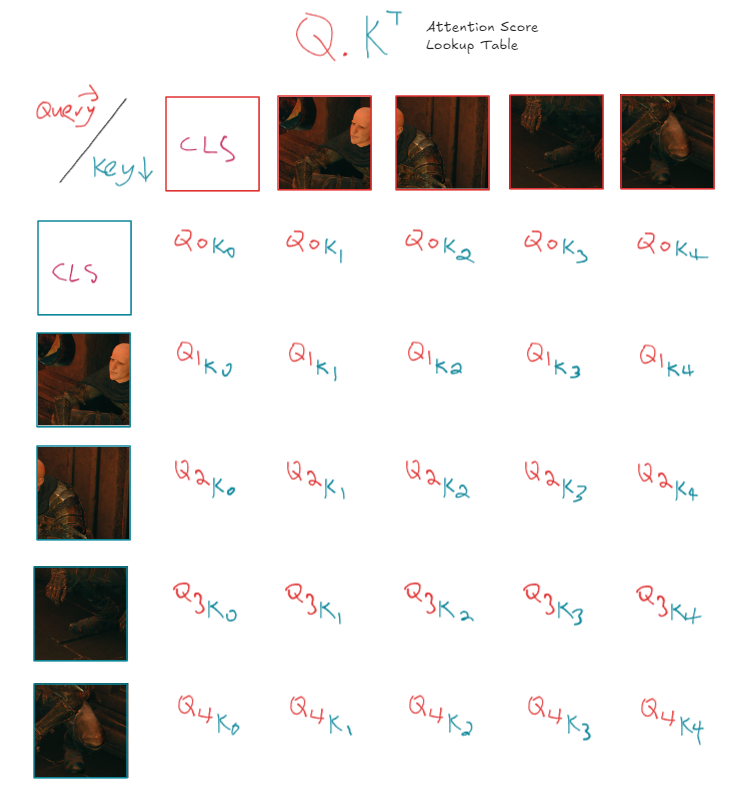
\includegraphics[keepaspectratio]{C:/Users/v4m5HSjp7tk/Documents/YEWTEEBEE/msc/notes/Project Ideas/image-44.png}}

Multiplying these attention scores (Q.K transposed) with the Value
matrix gives us a lookup table containing the information of the patch
weighted by how much focus to give to it.

\textbf{Why a value matrix? Why is the key not enough?}\\
-\textgreater{} Might want to retrieve something else than what is your
search criterion/the query

\textbf{Why not query the value matrix directly? (Why do we need the
key?)}\\
Issue: V does not exist in the same latent space as Q and K if d{}
\textgreater{} d{}\\
-\textgreater{} Q and K come from one embedding, V comes from a separate
embedding.\\
Even if d{} = d{} ,\\
\textbf{K is specifically designed to compare against Q, V is designed
to hold information}, not measure similarity. V contains features that
should be retrieved after relevance is decided.

\textbf{Why a value matrix? Why not use the embedded patches
directly?}\\
\hspace{0pt}-\textgreater{} Allows for a more refined representation
(raw linear projection of patch vs features captured from it), lower
dimensionality equals cheaper computations.

\subparagraph{Scaled dot product
Attention}\label{scaled-dot-product-attention}

Now that we have a way to express how much each patch should
\textbf{attend to} (pay attention to, give more focus on) other patches
in the form of a QK{} lookup table, we would want to apply this
expression to the value matrix.

\textbf{What does QK{} . V tell us?}\\
We can think of it as weighting the value matrix based on attention
scores.\\
\pandocbounded{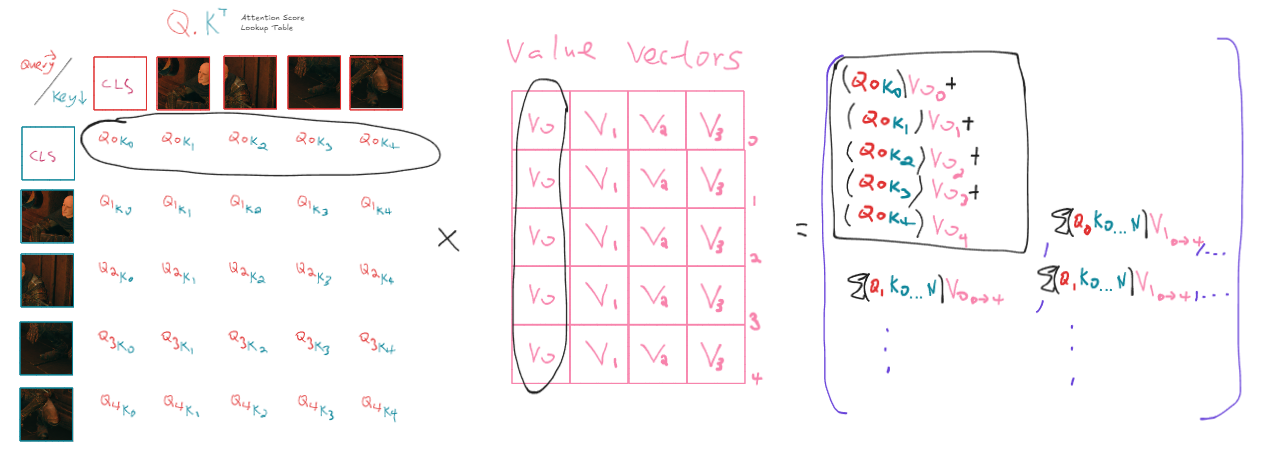
\includegraphics[keepaspectratio]{C:/Users/v4m5HSjp7tk/Documents/YEWTEEBEE/msc/notes/Project Ideas/image-69.png}}\\
Let each column of the value vector be a specific property that
describes each patch (e.g. how many round shapes?). Let each query be a
question (e.g. is there a bald head?) and each key be a descriptive list
(e.g. bald head, glove, armlet).

Patch 0 asks all the other patches: "Do you have what
I\textquotesingle m looking for?" The other patches replies with their
keys. If the key matches the query, the attention score is high.
Otherwise, the attention score is small or in the negatives.

We can see that, query-key matches increase the value of V0, while
query-key mismatches penalize the value of V0.

Thus, the first value (top left) of the weighted value matrix scales
property V0 for all patches by how much all the other patches satisfy
the query of patch 0.

The final representation of property 0 of patch 0 becomes a
\textbf{weighted combination} of its original value \textbf{plus} the
magnitude of that same property in other patches scaled by how much the
other patches satisfy the query of patch 0.

\textbf{Scaling the attention weights}\\
There are some adjustments to be made so that the scores serve better as
weights:

\begin{enumerate}
\tightlist
\item
  The attention scores are in the range of -inf to inf. This would put
  the scaling of the value matrix out of whack. We want this scaling to
  be in the range of 0 to 1 instead.
\end{enumerate}

\begin{itemize}
\tightlist
\item
  -\textgreater{} We do this by applying SoftMax to rescale the
  attention scores.
\end{itemize}

\begin{enumerate}
\tightlist
\item
  Softmax is sensitive to the magnitude of differences, rather than the
  magnitude of ratios (many large numbers, one small number = many 1s or
  near 1s and a 0). If the numbers are too close together, it messes
  with gradient calculations.
\end{enumerate}

\begin{itemize}
\tightlist
\item
  -\textgreater To fix this, we divide all values in the QK{} lookup
  table by the root of the key/query dimension.\\
  Together, we call it scaled dot product attention, which is a
  fundamental mechanism behind transformers.
\end{itemize}

\pandocbounded{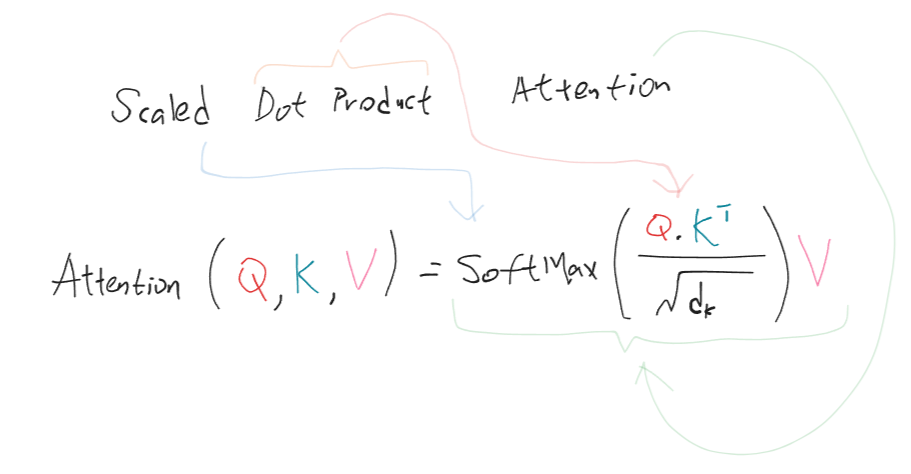
\includegraphics[keepaspectratio]{C:/Users/v4m5HSjp7tk/Documents/YEWTEEBEE/msc/notes/Project Ideas/image-59.png}}

\textbf{Putting it All Together}\\
\pandocbounded{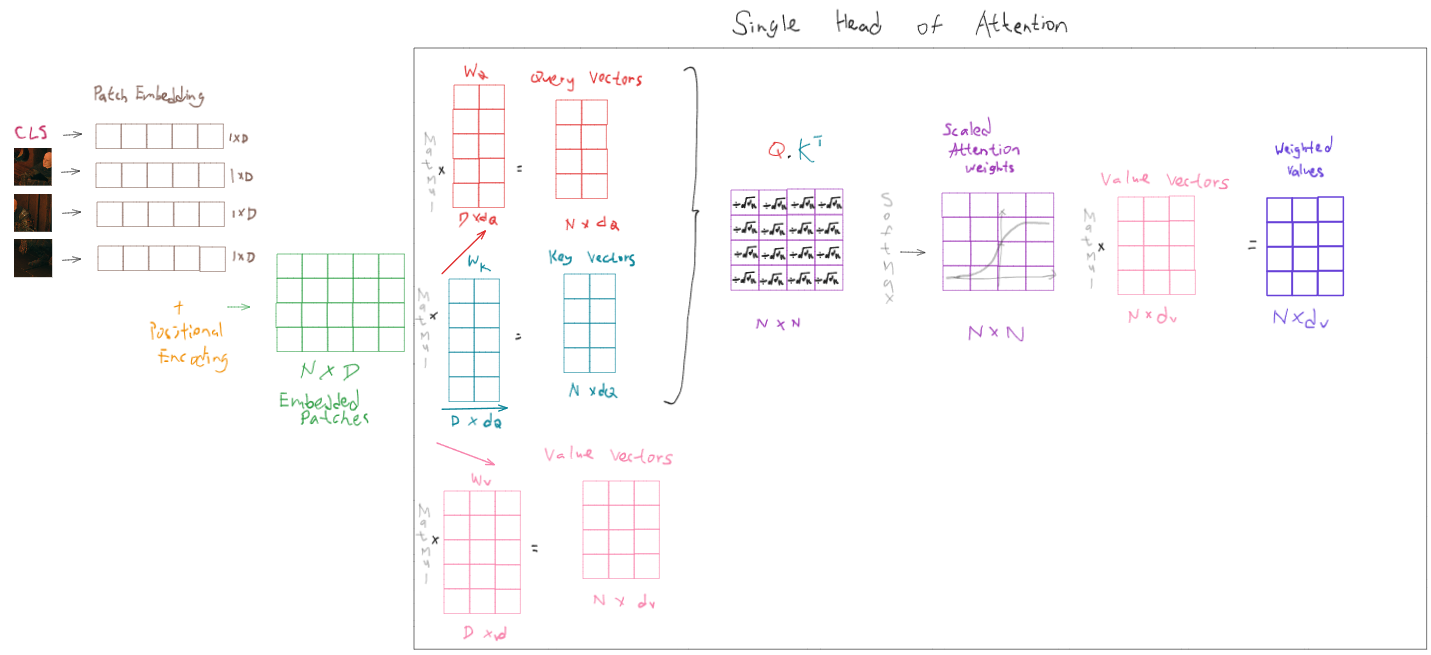
\includegraphics[keepaspectratio]{C:/Users/v4m5HSjp7tk/Documents/YEWTEEBEE/msc/notes/Project Ideas/image-73.png}}

\paragraph{Doing it in Parallel: Multi-headed
Attention}\label{doing-it-in-parallel-multi-headed-attention}

Multi-head self-attention applies self-attention (one head of attention)
multiple times at once in parallel, each head having its own key, query
and value transformations of the same input. The output of these heads
are combined at the end.\\
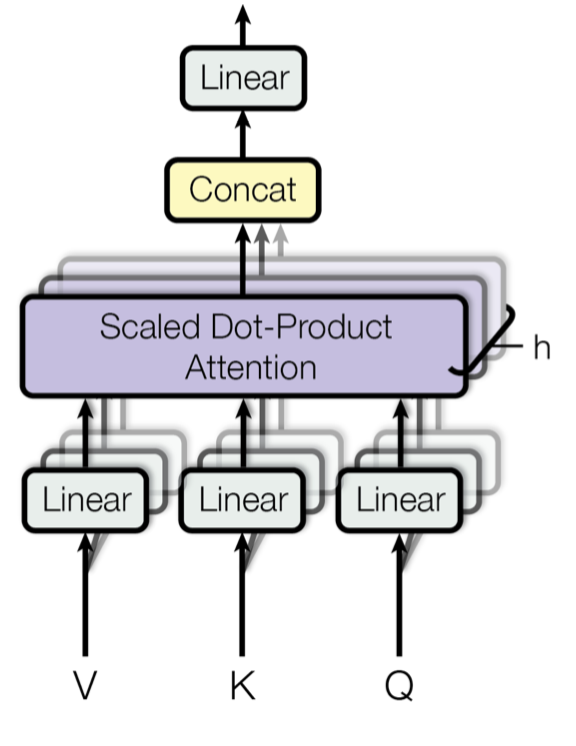
\includegraphics[width=3.36458in,height=4.35417in]{C:/Users/v4m5HSjp7tk/Documents/YEWTEEBEE/msc/notes/Project Ideas/image-75.png}

\textbf{Why multiple heads of attention?}\\
-\textgreater{} More descriptive power\\
Each head may focus on a specific aspect of an image (e.g. one head
learns shape, one head learns texture). i.e., Each head learns its own
lower-scale feature map (Q, K, V) corresponding to a specific feature as
opposed to one all-encompassing map.

\textbf{Idea: Multi-Head Attention (MHA) in Transformers is Analogous to
Multiple Kernels in CNNs}\\
\pandocbounded{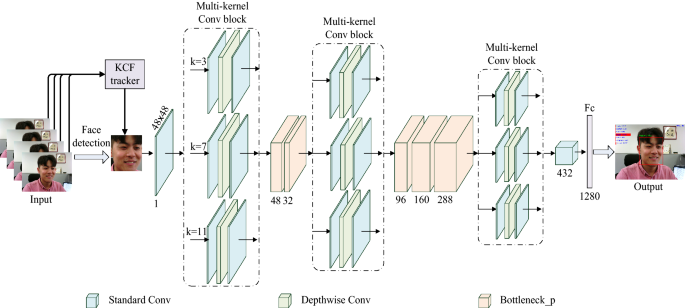
\includegraphics[keepaspectratio]{C:/Users/v4m5HSjp7tk/Documents/YEWTEEBEE/msc/notes/Project Ideas/image-76.png}}\\
Similar to multi-convolutional kernels (filters) in CNNs: process the
same input but extract different types of features, each with their own
weights.\\
However how they learn differently. CNN features get increasingly more
global as hierarchy (how far a layer is from the first) increases. ViT
features can be global from the start.

\subparagraph{Multi-head Attention
Implementation}\label{multi-head-attention-implementation}

Output value matrices from each attention head is concatenated together
dimension-wise, stacking the attention weighted values for each patch.

The concatenated output is projected back to the dimension of the
embedded patches (back to the same dimension as the input to each
attention head).

\pandocbounded{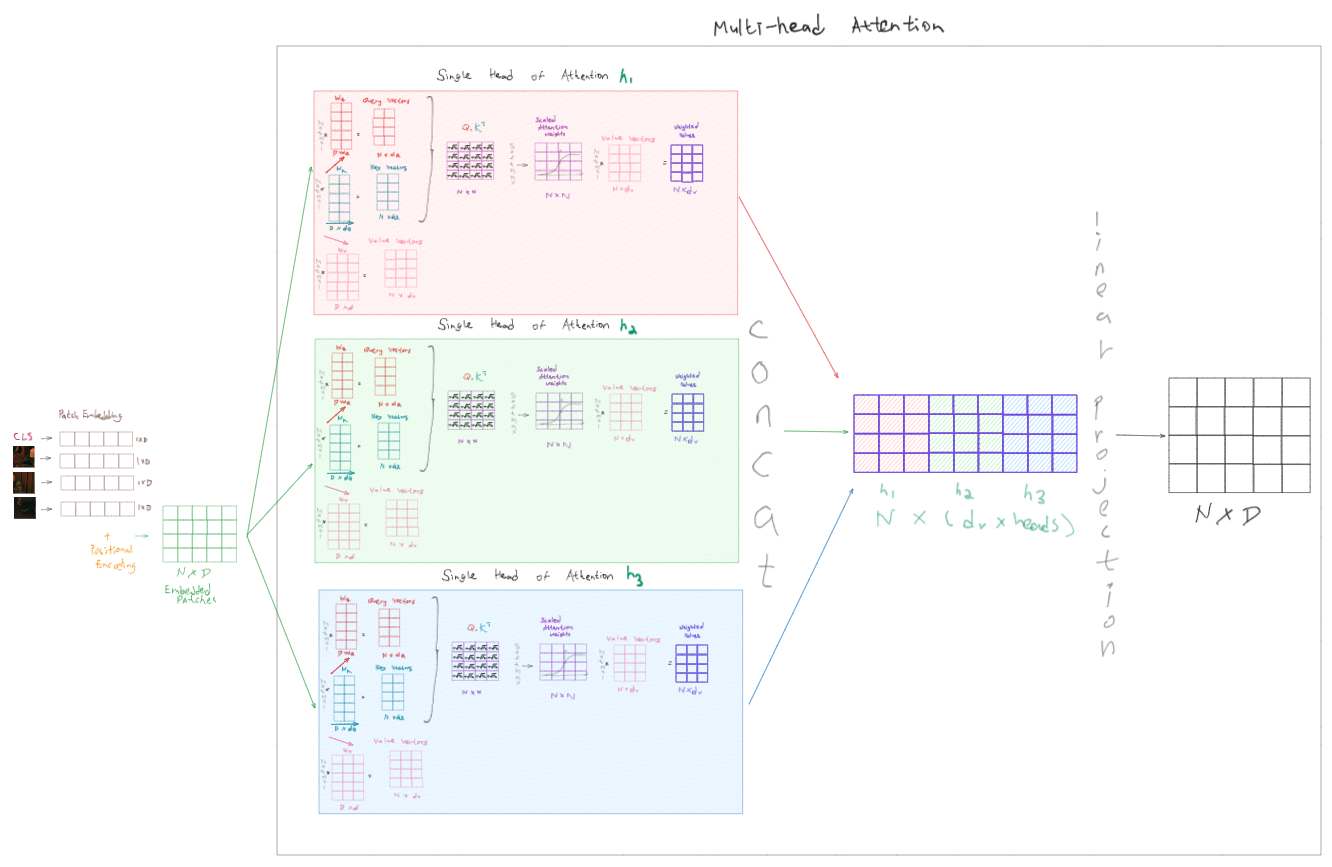
\includegraphics[keepaspectratio]{C:/Users/v4m5HSjp7tk/Documents/YEWTEEBEE/msc/notes/Project Ideas/image-80.png}}

What is the purpose of the final linear projection?\\
-\textgreater{} Combine the outputs from different heads into a single
representation, mixing the information\\
-\textgreater{} Easier implementation of residual connections

\paragraph{Parallelization}\label{parallelization}

In practice, we use 4-rank tensors to parallelize the math of the
attention heads.\\
\pandocbounded{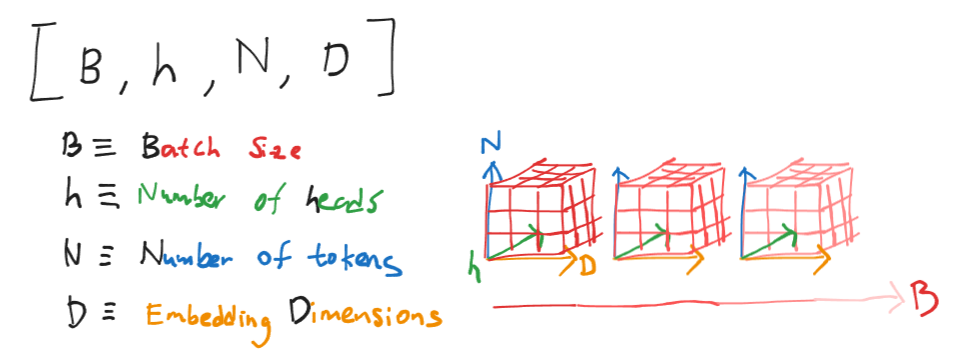
\includegraphics[keepaspectratio]{C:/Users/v4m5HSjp7tk/Documents/YEWTEEBEE/msc/notes/Project Ideas/image-83.png}}

Lets say we have a 32 x 32 image and choose 16 x 16 as the patch size.
That leaves us with N=5.\\
\pandocbounded{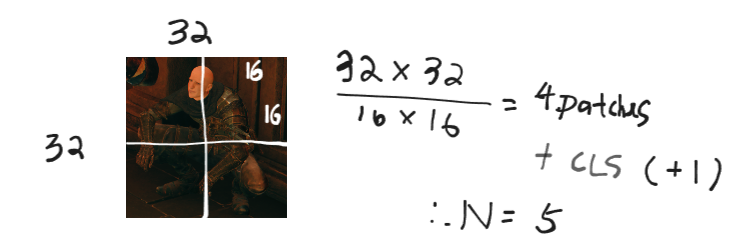
\includegraphics[keepaspectratio]{C:/Users/v4m5HSjp7tk/Documents/YEWTEEBEE/msc/notes/Project Ideas/image-84.png}}

Accounting for RGB, that gives us a {[}5 x 768{]} 2D tensor\\
\pandocbounded{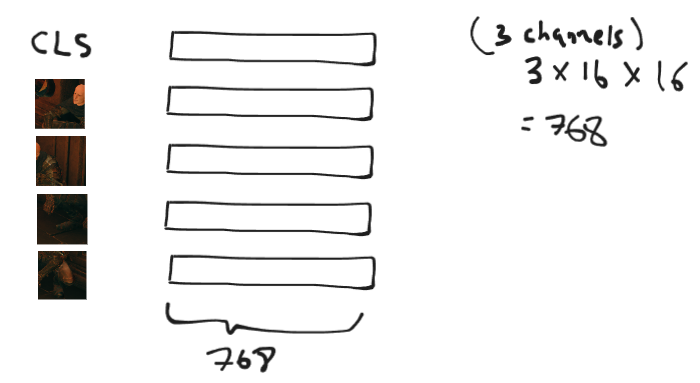
\includegraphics[keepaspectratio]{C:/Users/v4m5HSjp7tk/Documents/YEWTEEBEE/msc/notes/Project Ideas/image-85.png}}

We let embedding dimension D = 128\\
\pandocbounded{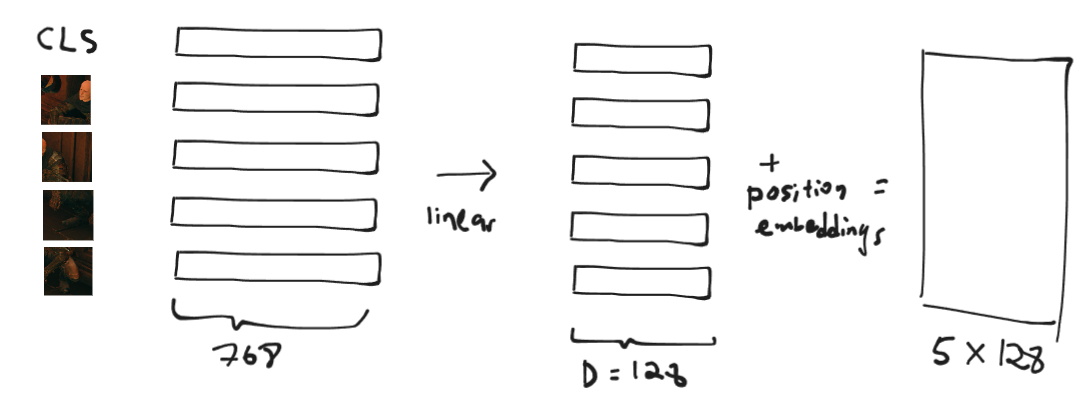
\includegraphics[keepaspectratio]{C:/Users/v4m5HSjp7tk/Documents/YEWTEEBEE/msc/notes/Project Ideas/image-88.png}}

Since we will be training in batches, we\textquotesingle ll introduce
batch dimension B.\\
We let d{}, d{} and d{} be = 32. That\textquotesingle s 96 weights per
attention head. We are using 4 attention heads, h = 4.
That\textquotesingle s a total of 384 weights per head.\\
In Pytorch\textquotesingle s ViT implementation, one big linear.nn is
used for the combined q,k,v weights for all heads.\\
\pandocbounded{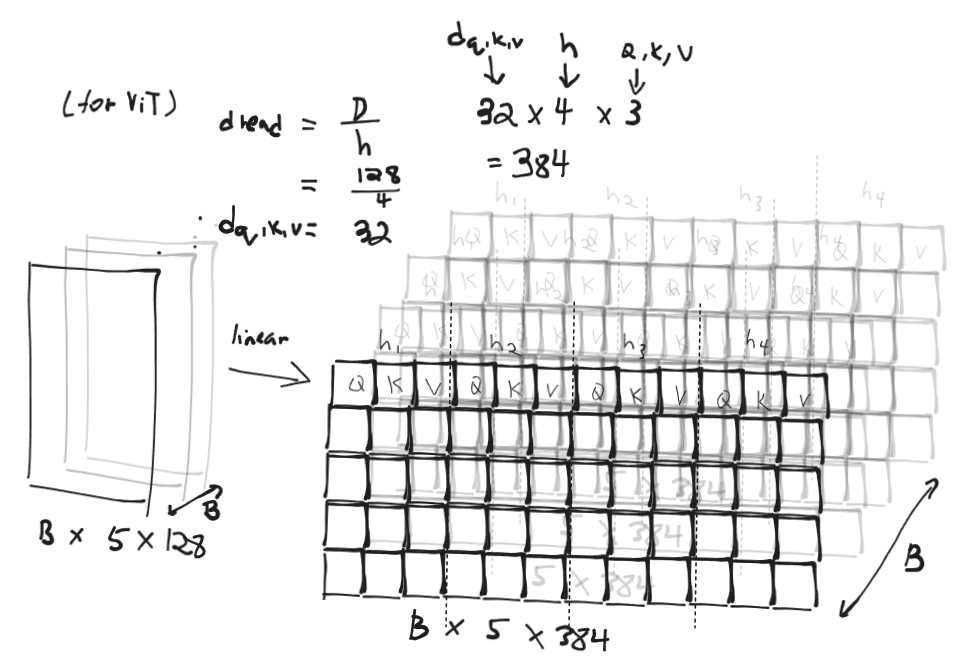
\includegraphics[keepaspectratio]{C:/Users/v4m5HSjp7tk/Documents/YEWTEEBEE/msc/notes/Project Ideas/image-92.png}}

The resulting matrix after applying the weights is then reshaped into
individual matrices along the head dimension.\\
\pandocbounded{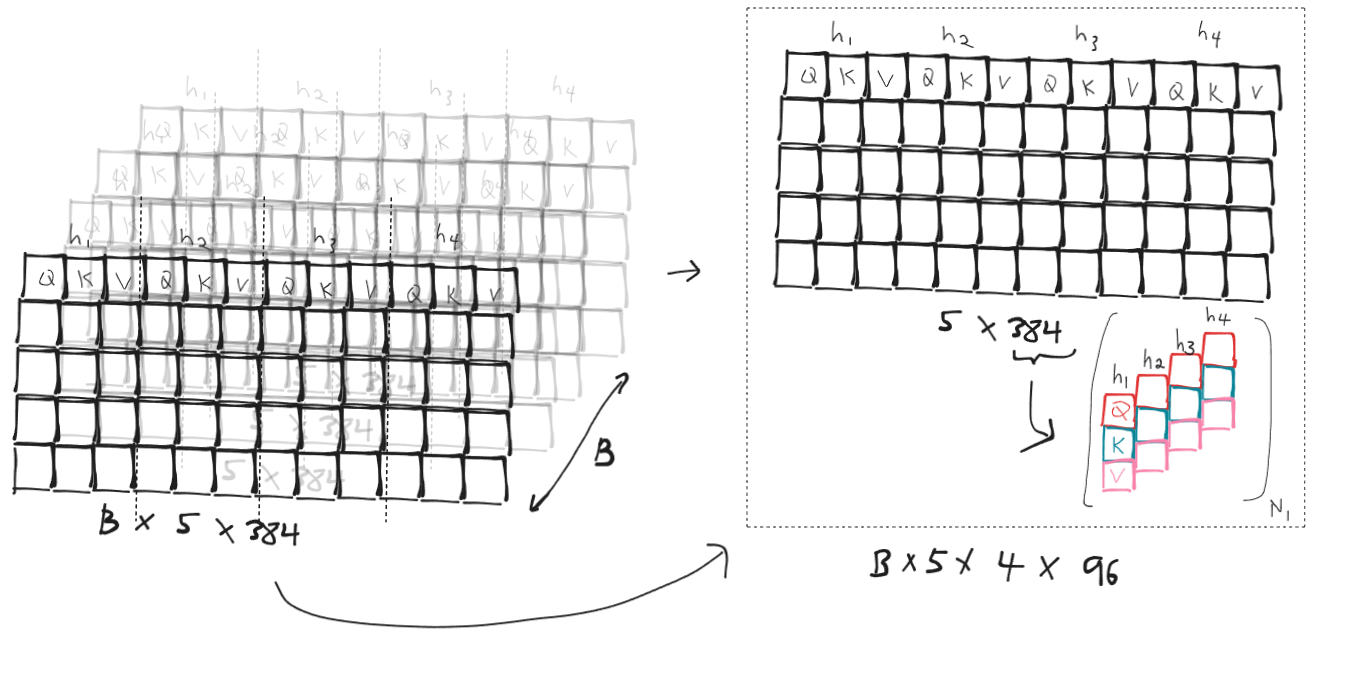
\includegraphics[keepaspectratio]{C:/Users/v4m5HSjp7tk/Documents/YEWTEEBEE/msc/notes/Project Ideas/image-94.png}}\\
\pandocbounded{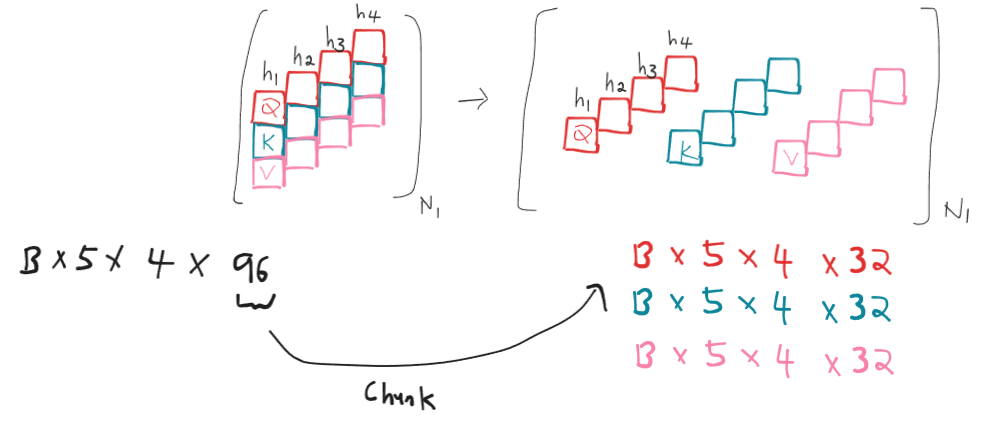
\includegraphics[keepaspectratio]{C:/Users/v4m5HSjp7tk/Documents/YEWTEEBEE/msc/notes/Project Ideas/image-96.png}}

In applying scaled dot product attention, we get the weighted values.
They are then concatenated (flattened).\\
\pandocbounded{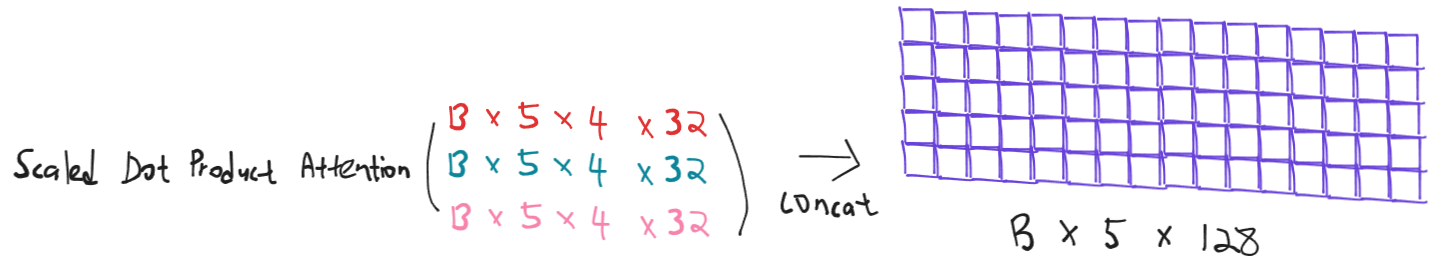
\includegraphics[keepaspectratio]{C:/Users/v4m5HSjp7tk/Documents/YEWTEEBEE/msc/notes/Project Ideas/image-100.png}}

We apply the final linear projection.\\
\pandocbounded{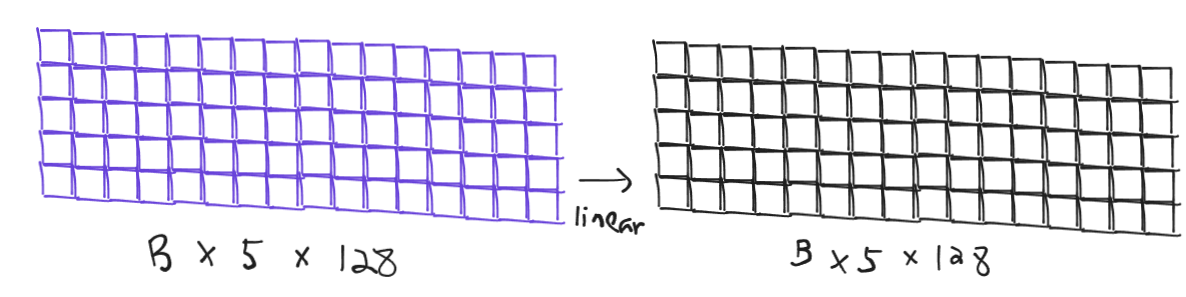
\includegraphics[keepaspectratio]{C:/Users/v4m5HSjp7tk/Documents/YEWTEEBEE/msc/notes/Project Ideas/image-101.png}}

We can thus see that in practice, multi-head self-attention is no more
expensive than single-head given the low-rankness of the transformations
we apply.

\paragraph{Multi-Layer Perceptron}\label{multi-layer-perceptron}

The output multi-head attention linear projection is inputted to a MLP.
All the operations so far are considered entirely linear operations
(even though information between tokens are mixed by the end of MHA).
The MLP block introduces non-linear activations\textsuperscript{{[}1{]}}
such that the model learns non-linear representations, allowing for the
"bending" of feature space. This breaks the linearity and can
exponentially increases \textsuperscript{{[}2{]}} model expressiveness.

Non-Linearity

The composition of one or more linear functions is itself a linear
function. A neural network using only linear activations can be
rewritten as a linear function, no matter how wide or deep the neural
network.\\
\pandocbounded{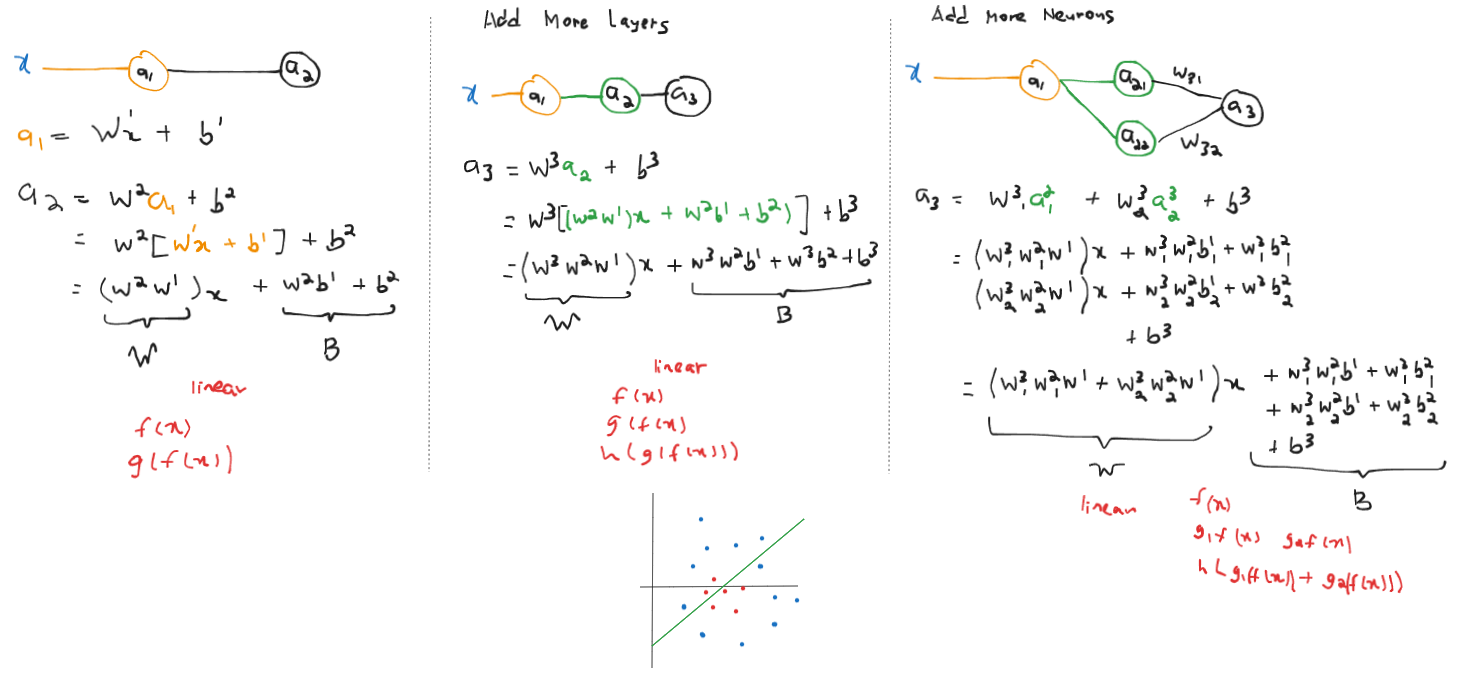
\includegraphics[keepaspectratio]{C:/Users/v4m5HSjp7tk/Documents/YEWTEEBEE/msc/notes/Project Ideas/image-128.png}}

If we add a non-linear activation function, we introduce non-linearity.
Some of the more common non-linear functions tanh and sigmoid which
curves, and ReLU, which is piecewise linear (thus non-linear).\\
\pandocbounded{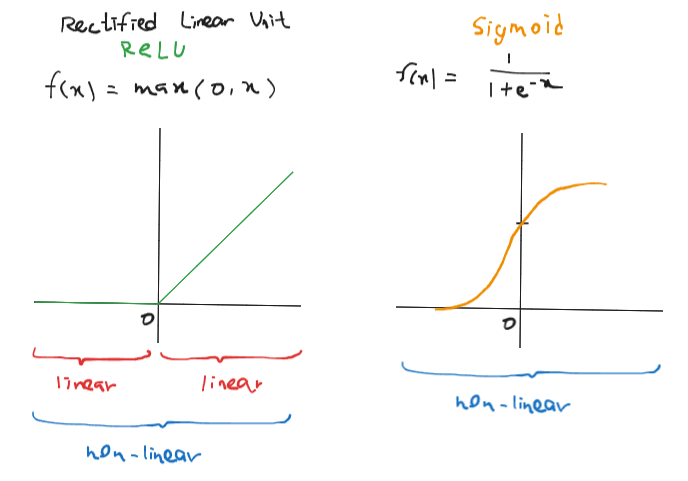
\includegraphics[keepaspectratio]{C:/Users/v4m5HSjp7tk/Documents/YEWTEEBEE/msc/notes/Project Ideas/image-129.png}}

ReLU is especially common in machine learning as it

\begin{enumerate}
\tightlist
\item
  Is just a simple max operation, super easy to compute (and its
  derivatives are just 1 or 0)
\item
  Introduces sparsity as the output for \textless0 values is 0. These 0
  activations are equivalent to inactive neurons.\\
  ReLU on a deep enough neural network can perform piecewise
  approximations of non-linear functions and decision boundaries.
  \hl{Breaking linearity allows for non-linear representations,} which
  is one of the main motivations for having non-linear activations in
  the transformer MLP.
\end{enumerate}

Video Demonstration of Non-Linear Approximation:\\
\url{https://www.youtube.com/watch?v=joA6fEAbAQc}

Interactive Demonstration of Neural Networks with Different Activation
Functions:\\
\url{https://playground.tensorflow.org/}

linear activations = only can have linear boundary (single line)\\
\pandocbounded{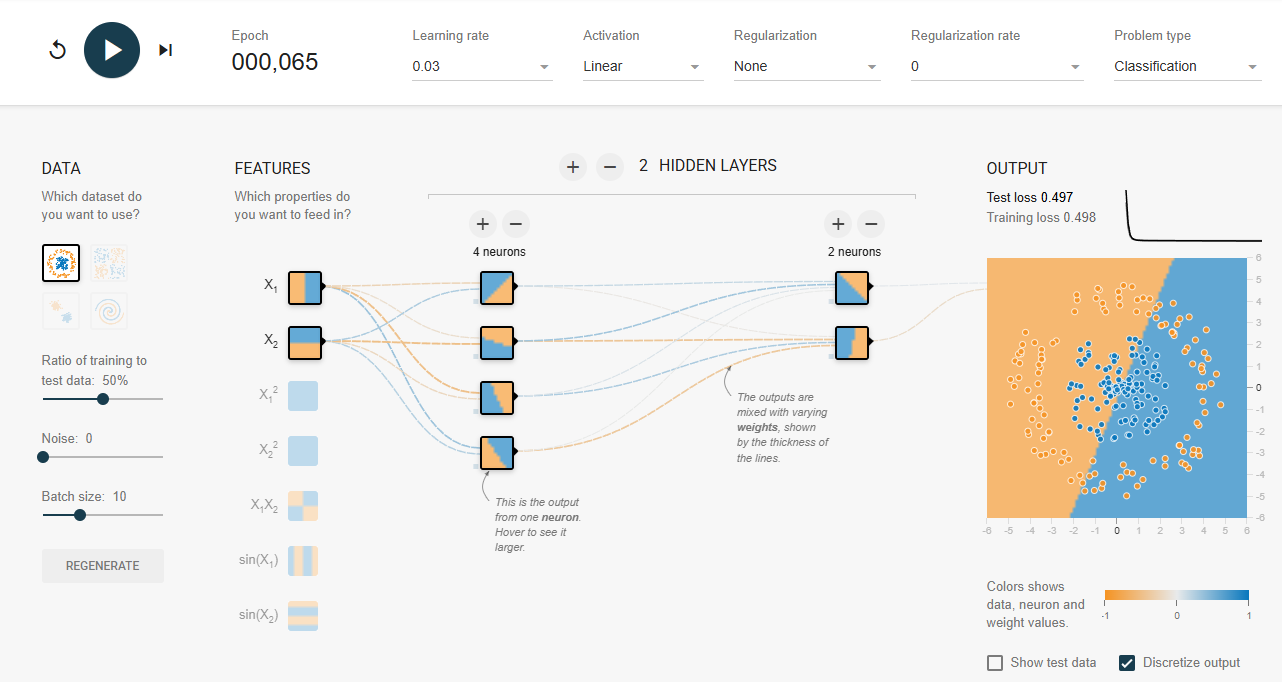
\includegraphics[keepaspectratio]{C:/Users/v4m5HSjp7tk/Documents/YEWTEEBEE/msc/notes/Project Ideas/image-124.png}}\\
ReLU allows for the bending of the decision boundary\\
\pandocbounded{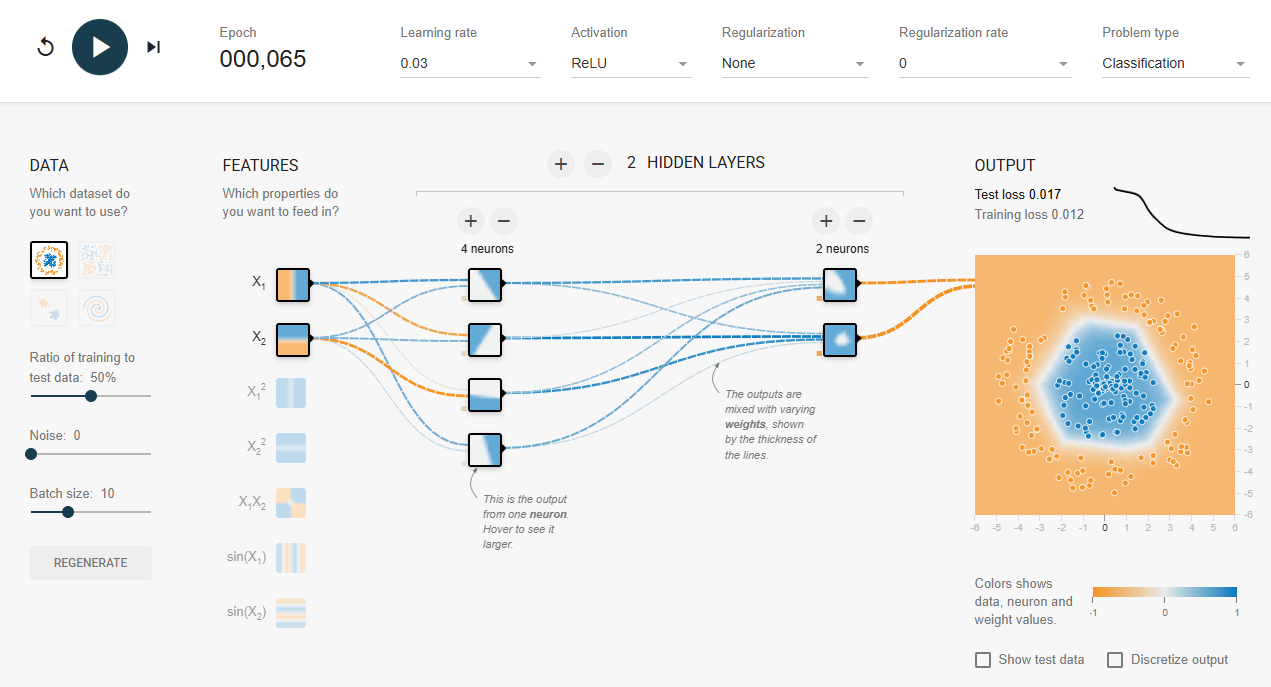
\includegraphics[keepaspectratio]{C:/Users/v4m5HSjp7tk/Documents/YEWTEEBEE/msc/notes/Project Ideas/image-125.png}}

A simple two-layer MLP with GELU activation in between is used in the
Transformer encoder. An expansion factor of 4 is used where the depth of
the first layer is 4D. The second layer shrinks the dimensionality back
to D.\\
\pandocbounded{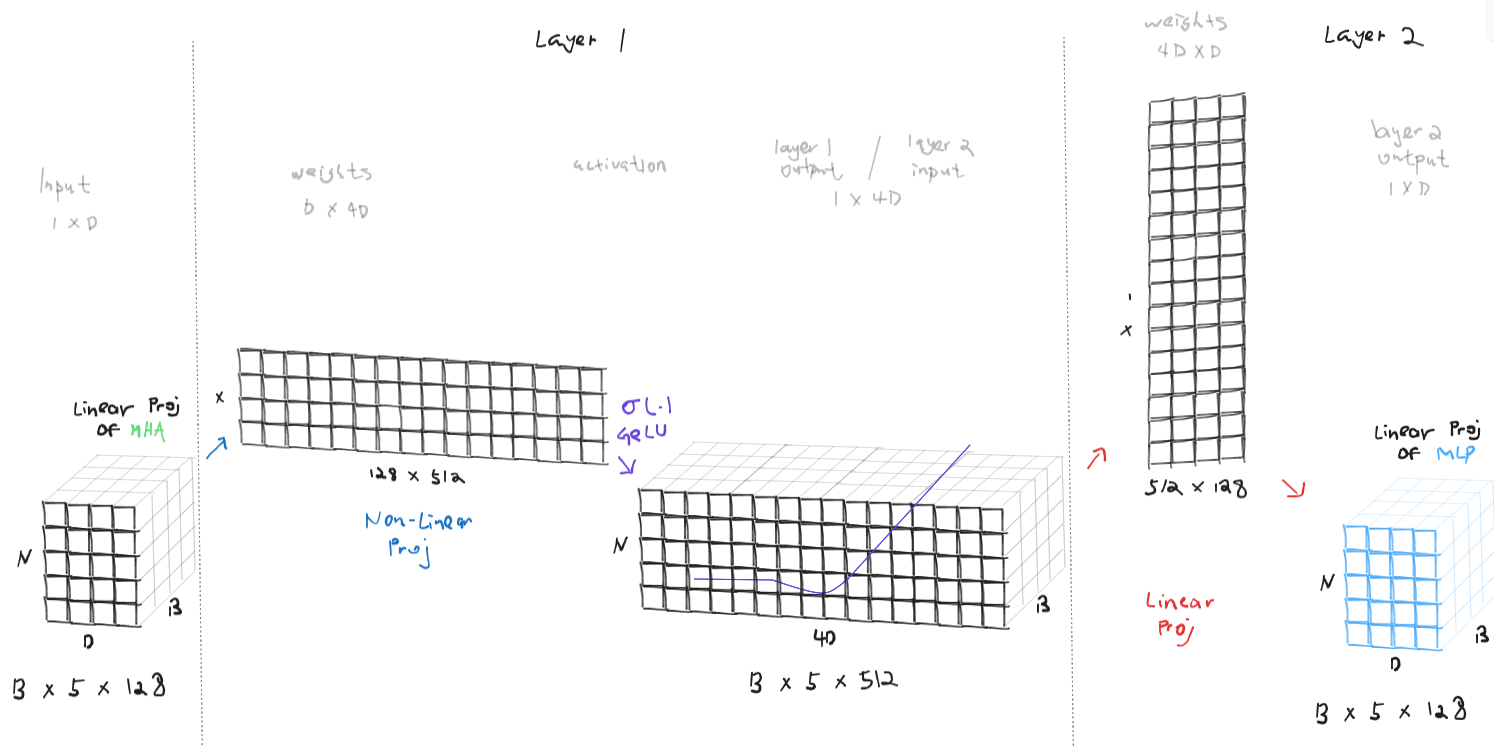
\includegraphics[keepaspectratio]{C:/Users/v4m5HSjp7tk/Documents/YEWTEEBEE/msc/notes/Project Ideas/image-134.png}}

\subparagraph{Gaussian Error Linear Unit (GeLU)
Activation}\label{gaussian-error-linear-unit-gelu-activation}

The GeLU non-linearity weights inputs by their percentile in the
cumulative distribution function of a Gaussian distribution. In the case
of transformers, the range of values for a given input token is
what\textquotesingle s being weighted. That is:-

\begin{itemize}
\tightlist
\item
  For \textbf{very negative x:} Φ(x)≈ 0 \textbar{} small number *
  negative x \textbar{} ≈0
\item
  For \textbf{very positive x}: Φ(x)≈ 1 \textbar{} x\\
  Therefore, Φ(x) is linear for large values of x, softly scales down
  small positive values, softly scales up small negative values and
  nullifies large negative values.\\
  \pandocbounded{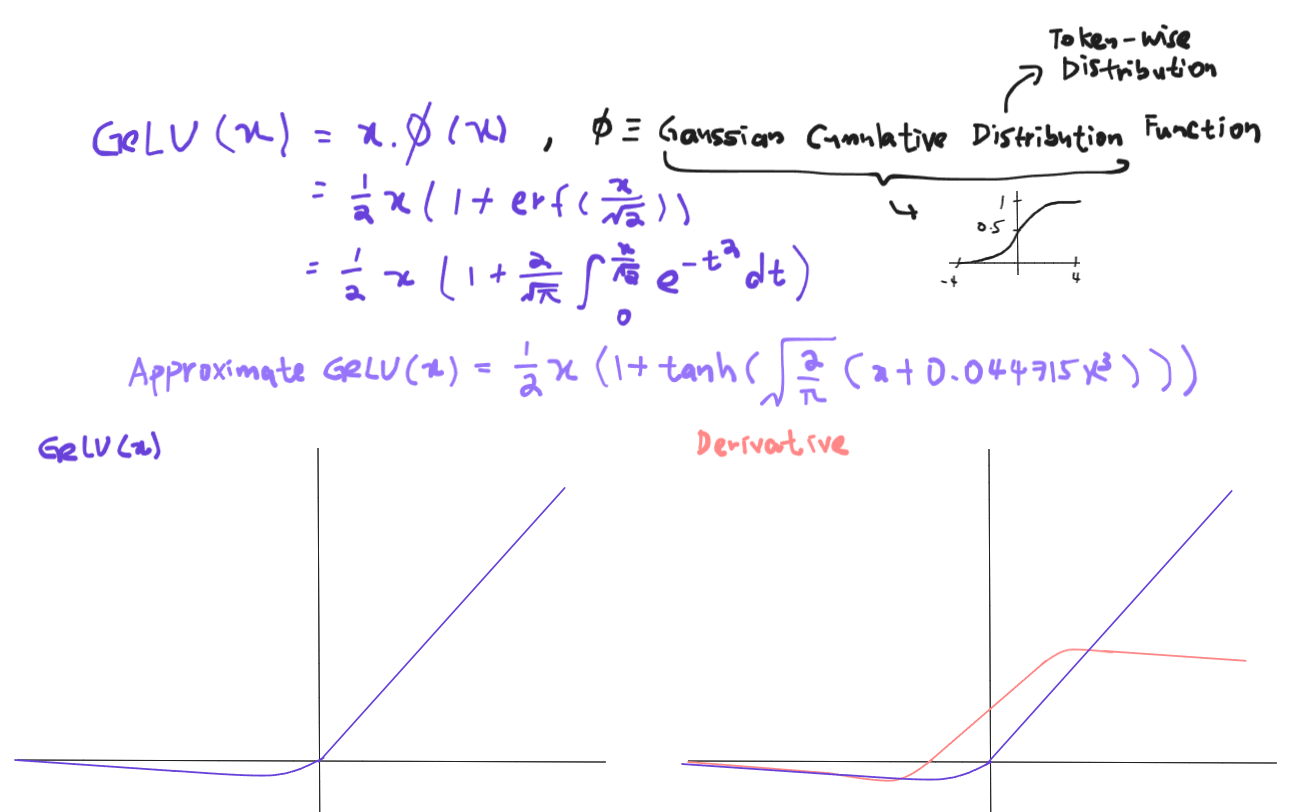
\includegraphics[keepaspectratio]{C:/Users/v4m5HSjp7tk/Documents/YEWTEEBEE/msc/notes/Project Ideas/image-137.png}}
\end{itemize}

Why GeLU?

GeLU is smooth and differentiable in all ranges, allowing gradients
(although small) in negative range. Compared to ReLU with only 1 or 0 as
derivatives, GeLU can push weights in more directions. It also mitigates
the dying RELU problem, negative inputs still give a small non-zero
output and gradient rather than 0.

GELU is non-monotonic, which means its output does not only increase or
decrease (i.e., the valley in the graph). In theory, this can translate
to dynamically filtering out small unhelpful signals. The activation is
much more expressive compared to ReLU.

GELUs are used in~GPT-3,~BERT, and most other Transformers.

\paragraph{Extra tricks for stability}\label{extra-tricks-for-stability}

Since transformers are highly parallelizable, we often take advantage of
the saved compute time by scaling up the model. Thus, we want the model
to maintain stability and efficiency as scale increases.

\subparagraph{LayerNorm}\label{layernorm}

\pandocbounded{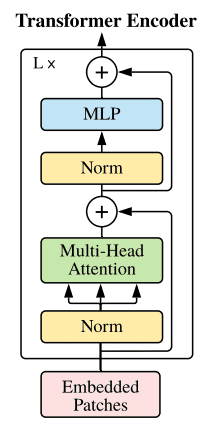
\includegraphics[keepaspectratio]{C:/Users/v4m5HSjp7tk/Documents/YEWTEEBEE/msc/notes/Project Ideas/image-81.png}}\\
Batch Normalization is a trainable method known to speed up convergence
and improve stability in neural networks. Initially proposed to solve
internal covariate shifts, it is now believed that the smoothing effect
brought upon by normalization (especially during backpropagation) is the
stronger proponent of the improvements. BatchNorm normalizes across the
batch dimension.

Covariate Shift

\textbf{Covariate shift} describes a change where\texttt{P(X)}changes
but \texttt{P(Y\textbar{}X)} remains the same. e.g., During Ramadan, the
odds of a shop being closed at Iftar is 0.9. In the context of a whole
year, the odds are 0.075. A model trained during Ramadan would have
\texttt{P(closed\textbar{}X)} = 0.9, and perform pathetically bad when X
is the whole year. \textbf{Internal covariate shift} brings this concept
to training neural networks, where X in this case is inputs from
previous layers. The randomness of initial weight values and batch
selection leads to instability in inputs.

BatchNorm sucks

BatchNorm is insidious for causing bugs in transformers. BatchNorm needs
to look at all samples in the batch to compute mean and variance,
creating a synchronization bottleneck when training across multiple
GPUs. BatchNorm also assumes I.I.D. of which the opposite is often
encountered in practical scenarios AND hard to achieve when sampling
randomly. On top of that, BatchNorm is expensive to compute and causes
look-ahead issues for sequence models. We have since phased out of using
BatchNorm, favouring LayerNorm and RMSNorm instead.

LayerNorm in transformers normalizes across the features/embeddings of
each token. The name itself is misleading, as LayerNorm in CNN
normalizes across the entire image. LayerNorm is actually similar to
InstanceNorm for transformers, the terminology has just been brought
forward from preceding works.

Comparing Norms

\pandocbounded{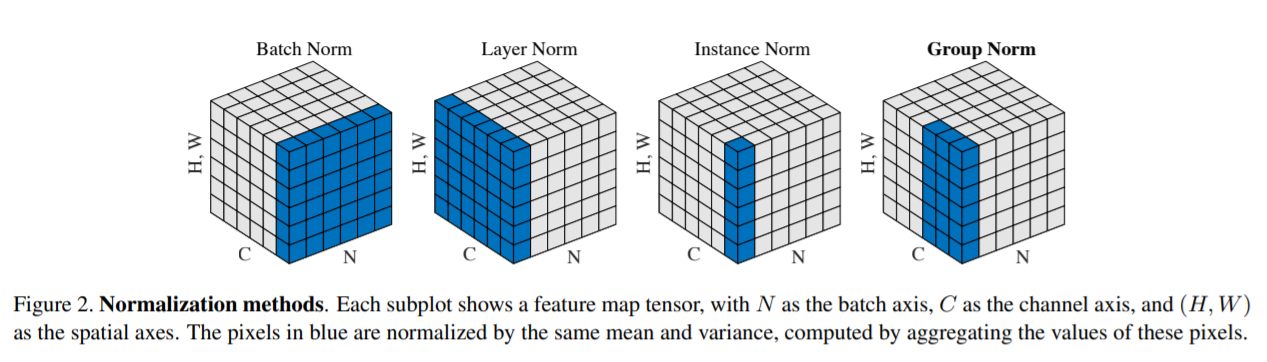
\includegraphics[keepaspectratio]{C:/Users/v4m5HSjp7tk/Documents/YEWTEEBEE/msc/notes/Project Ideas/image-109.png}}

LayerNorm re-centres each patch embedding of each token into a standard
normal distribution. A small constant ϵ is added to the denominator for
numerical stability (prevent div 0 or very small values). Two learnable
affine parameters γ and β are typically used to allow for a more
flexible representation of the distribution.\\
\pandocbounded{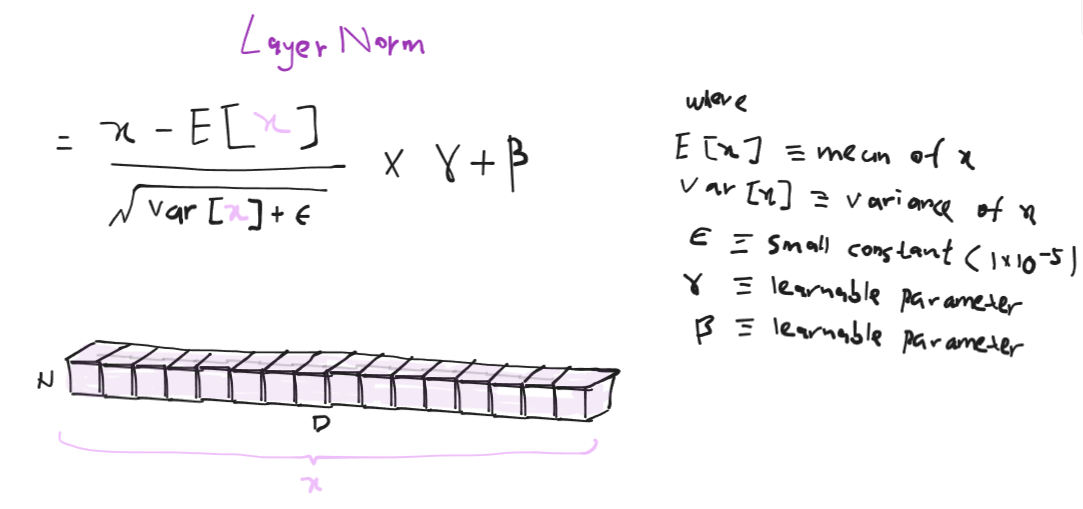
\includegraphics[keepaspectratio]{C:/Users/v4m5HSjp7tk/Documents/YEWTEEBEE/msc/notes/Project Ideas/image-103.png}}

γ controls the scale of the distribution, β controls the shift\\
\pandocbounded{\includegraphics[keepaspectratio]{C:/Users/v4m5HSjp7tk/Documents/YEWTEEBEE/msc/notes/Project Ideas/image-105.png}}

LayerNorm is performed twice in a transformer encoder block: -

\begin{enumerate}
\tightlist
\item
  Once on the embedded patches before multi-head attention
\item
  Once more on the output of the multi-head attention before feeding to
  MLP\\
  \pandocbounded{\includegraphics[keepaspectratio]{C:/Users/v4m5HSjp7tk/Documents/YEWTEEBEE/msc/notes/Project Ideas/image-108.png}}
\end{enumerate}

PreNorm vs PostNorm

ViT uses Pre-LayerNorm, where LayerNorm is performed before the
Multi-Head Attention and MLP as well as the summation from residual
connection proceeding them. This is a reordering of steps from the
original transformer paper, which uses Post-LayerNorm. In
Post-LayerNorm, LayerNorm takes place after the summation and preceding
MHA/MLP.

Pre-LN supersedes Post-LN in transformers. Putting LN after the residual
connections makes the LN effectively LN(activations{} + x)), resulting
in expected gradients of the parameters near the output layer to
explode. Early in training, weights are small → sublayers produce small
outputs. So most of the signal comes from the residual (i.e., x + ε). As
LayerNorm is applied, and it tries to normalize the tiny activations to
unit variance. This artificially inflates the scale of outputs (and
gradients) especially in later layers near the output. A practical
solution was to have a warm-up step that varies the learning rate from
small to big and back to small at the initialization.

Pre-LN removes the requirement for the warm-up step completely. The
residual path of the Transformer is kept clean, and each sublayer
receives normalized input. This results in the gradients being
well-behaved at initialization and positively improves training
stability.

\subparagraph{Residual Connections}\label{residual-connections}

Issues with Deep Neural Networks

\textbf{Initialization}\\
Deep neural networks have been notoriously harder to train as the number
of layers increase. At initialization, random weights and activations
from each layer progressively alter the input randomly as it propagates
from layer to layer. At the final layers, the output may differ greatly
from the initial input to the point that it is just random noise. This
makes the initial training of the network result in much slower
convergence compared to a shallow network, as the loss function wanders
around randomly.\\
\pandocbounded{\includegraphics[keepaspectratio]{C:/Users/v4m5HSjp7tk/Documents/YEWTEEBEE/msc/notes/Project Ideas/image-117.png}}

\textbf{Vanishing and Exploding Gradients}\\
When we calculate loss in a large neural network, we get increasingly
longer chains of partial derivatives which contains values that are
bounded to\textless1 (derivatives of common activations ReLU, sigmoid,
etc.). When we multiply many \textless1 values, we get a really small
number. The further back in the layers we go, the longer the chain and
smaller the loss. If the loss gets too close to 0 for one layer, the
layers before it will not be updated (0 loss = correct prediction).
Learning is thus haltered for these preceding layers. The opposite is
also true where gradients are too big and cause a cascade effect of
exploding weights.

ResNets are the Solution

\pandocbounded{\includegraphics[keepaspectratio]{C:/Users/v4m5HSjp7tk/Documents/YEWTEEBEE/msc/notes/Project Ideas/image-116.png}}

ResNets solve the scalability issue in deep neural networks by using
skip connections via addition.\\
We simply add the input of a layer to the output of a non-immediate
following layer. The residual block is structured to learn adjustments
\texttt{F(x)} to the input \texttt{x}, i.e., the \textbf{residuals}
rather than synthesize a direct mapping.\\
\pandocbounded{\includegraphics[keepaspectratio]{C:/Users/v4m5HSjp7tk/Documents/YEWTEEBEE/msc/notes/Project Ideas/image-114.png}}

\textbf{Effect: Not all Layers has to be Useful}\\
Residual connections fundamentally allow deeper models to perform at
least as well as a shallower counterpart. If the two layers in the
diagram above is not needed, the model simply has to learn
\texttt{F(x)\ =\ 0} rather than \texttt{F(x)\ =} a{}, which is much,
much easier. As a result, ResNets behave like an ensemble of shallow
networks.

\textbf{Effect: Helps with Vanishing Gradients}\\
The gradients in the direct network is calculated as a multiplicative
chain of partial derivatives, whereas the residual network passes its
gradient to earlier layer no matter how small the multiplication of
partial differentials become (we also see it as creating a new direct
path for the residual block loss to flow to the residual block input).\\
\pandocbounded{\includegraphics[keepaspectratio]{C:/Users/v4m5HSjp7tk/Documents/YEWTEEBEE/msc/notes/Project Ideas/image-119.png}}

\textbf{Effect: Smoothing the Loss Landscape}\\
Residual connections effectively smoothens the loss landscape and
simplifies optimization. It has been theorized that residual connections
bypass conflicting layers (layers that just add noise) in a neural
network.\textsuperscript{{[}3{]}} Skip connections allow the model to
fall back on the identity mapping if the neurons in some layers are not
helping.\\
\pandocbounded{\includegraphics[keepaspectratio]{C:/Users/v4m5HSjp7tk/Documents/YEWTEEBEE/msc/notes/Project Ideas/image-115.png}}

Residual Connections in Transformer Architectures

Going back to the need for scalability, Transformers can get really deep
especially considering they meant to run at scale. Residual connections
help with numerical stability and optimization. The connection connects

\begin{enumerate}
\tightlist
\item
  the unnormalized input to the MHA output,
\item
  unnormalized input and MHA output to the MLP output. In a way, we are
  reminding the MLP and MHA what the original input was.\\
  (Note: only residual connection, output is not passed to an activation
  function like in ResNets)\\
  \pandocbounded{\includegraphics[keepaspectratio]{C:/Users/v4m5HSjp7tk/Documents/YEWTEEBEE/msc/notes/Project Ideas/image-120.png}}
\end{enumerate}

\subparagraph{Stacking Multiple Layers of Transformer
Encoders}\label{stacking-multiple-layers-of-transformer-encoders}

Transformer Networks stack multiple transformer layers (also called
blocks) sequentially (encoder-only for ViT). The output for each layer
is taken as the input for the next layer.\\
\pandocbounded{\includegraphics[keepaspectratio]{C:/Users/v4m5HSjp7tk/Documents/YEWTEEBEE/msc/notes/Project Ideas/image-141.png}}

Effect of Stacking Layers

Stacking multiple layers enables the model to refine representations
hierarchically, analogous to adding depth to a CNN model. The earlier
layers in ViT learn to encode more local information, while later layers
encode more global information4.

Transformers use \textbf{pairwise} self-attention, which relates to
\textbf{one} token attending to \textbf{one} other token at a time. By
the time the embeddings reach the output, this information is mixed,
encoding global context. Attention in the second layer onwards is not
just pairwise patch attention anymore, but refined, mixed, and
aggregated information from all patches simultaneously. As we go from
layer to layer, the model learns more refined relationships and further
aggregate context across patches. Essentially, each patch's
representation becomes more contextually aware of other patches through
the successive layers. This leads to richer representations as
long-range dependencies are progressively refined when propagating
throughout layers.

As you stack additional encoder layers, the amount of complexity the
network can model grows.

Why Transformers require more data than CNNs

CNNs have an explicit locality bias in earlier layers due to how
kernelling works (each neuron sees a small receptive field at first,
later layers can see the pixels within the receptive fields of prior
layers).\\
ViT encodes the entire image from the start and don't have built-in
local-to-global hierarchy like CNNs. ViTs learn hierarchy implicitly
from data, which has shown to have a local-to-global hierarchy4. The
flexibility of ViTs to learn whatever hierarchical relationship it wants
leads to a requirement for more training data.

\pandocbounded{\includegraphics[keepaspectratio]{C:/Users/v4m5HSjp7tk/Documents/YEWTEEBEE/msc/notes/Project Ideas/image-143.png}}\\
Picture: The closer layers are to each other, the more similar. Opposite
applies. Implies local-to-global hierarchy.

\subparagraph{MLP Head (Classification
Head)}\label{mlp-head-classification-head}

The CLS token from the output of the final layer is passed to a linear
layer (MLP head/classification head). The MLP head has one layer. This
layer maps D to the number of classes, giving the probability
distribution logits for each class.\\
\pandocbounded{\includegraphics[keepaspectratio]{C:/Users/v4m5HSjp7tk/Documents/YEWTEEBEE/msc/notes/Project Ideas/image-145.png}}

\paragraph{Recap: Counting Parameters and Big
O}\label{recap-counting-parameters-and-big-o}

As a sanity check, lets obtain back the 86M params in the base ViT
model. The number of classes is 1000 for ImageNet, and there are 196 + 1
patches of 16 x 16.\\
\pandocbounded{\includegraphics[keepaspectratio]{C:/Users/v4m5HSjp7tk/Documents/YEWTEEBEE/msc/notes/Project Ideas/image-138.png}}

Looking back into the entire ViT architecture, we have the following
weights:-\\
\pandocbounded{\includegraphics[keepaspectratio]{C:/Users/v4m5HSjp7tk/Documents/YEWTEEBEE/msc/notes/Project Ideas/image-147.png}}

\textbf{Transformer Block}\\
x L layers of:

\begin{itemize}
\tightlist
\item
  x 12 heads of:

  \begin{itemize}
  \tightlist
  \item
    key, query, value weights \textbf{3 x D x d{}}
  \item
    linear projection weights \textbf{D x D}
  \end{itemize}
\item
  1st MLP layer weights \textbf{D x 4D}
\item
  2nd MLP layer weights \textbf{4D x D}
\end{itemize}

\textbf{MLP head}\\
CLS to number of classes weights \textbf{D x number of classes}

\textbf{Patch Embeddings}\\
Patch Embeddings projection weights \textbf{(Patch Size x 3) x D}\\
Learnable Positional Embeddings \textbf{N x D}

which shortens to:-\\
{}\strut \\
=12(12(3 x 768 x 64) + 768 x 768 + 2(4 x 768 x 768)) + (768 x 1000) +
3(16) x 768 + 768 x 768\\
=86,329,344\\
which is approximately 86M

\paragraph{Cross Attention}\label{cross-attention}

\begin{center}\rule{0.5\linewidth}{0.5pt}\end{center}

Gallbladder cancer detection with Focus Masked MAE\\
\url{https://openaccess.thecvf.com/content/CVPR2024/papers/Basu_FocusMAE_Gallbladder_Cancer_Detection_from_Ultrasound_Videos_with_Focused_Masked_CVPR_2024_paper.pdf}

learned locality

the model has to implicitly learn that pixels are in 2d

\begin{center}\rule{0.5\linewidth}{0.5pt}\end{center}

\begin{enumerate}
\item
  \phantomsection\label{fn-1-3a762d0062c52d14}
  \url{https://openreview.net/pdf?id=I8pdQLfR77}
\item
  \phantomsection\label{fn-2-3a762d0062c52d14}
  \url{https://arxiv.org/pdf/1606.05336}
\item
  \phantomsection\label{fn-3-3a762d0062c52d14}
  \url{https://arxiv.org/pdf/2103.04331}
\end{enumerate}

\end{document}
